
\chapter{METHODOLOGY}
\label{intro}
\vspace{-3em}
The first and foremost task of the research was image acquisition which contains components such as image collection, preprocessing, and augmentation. The research is divided into two phases - detection and prediction. The detection was conducted in two techniques: Training Individual Models and Ensemble Learning Approach. All combinations of trained models were evaluated and then a comparative analysis of the models was assessed. Similarly, the prediction phase followed the following workflow - image pairing and calculation of GVI difference, training of the selected RNN models, and evaluation of their performance to select the best performing and finally, predicting the future GVI difference using siamese model and the best performing RNN model. Figure \ref{fig:methodology1} illustrates the methodology followed for detection while Figure \ref{figures/pred_method.png} portrays the procedure of the prediction phase. All the proceedings are elaborately discussed below.

\begin{figure}
\centering
% \vspace{-30mm}
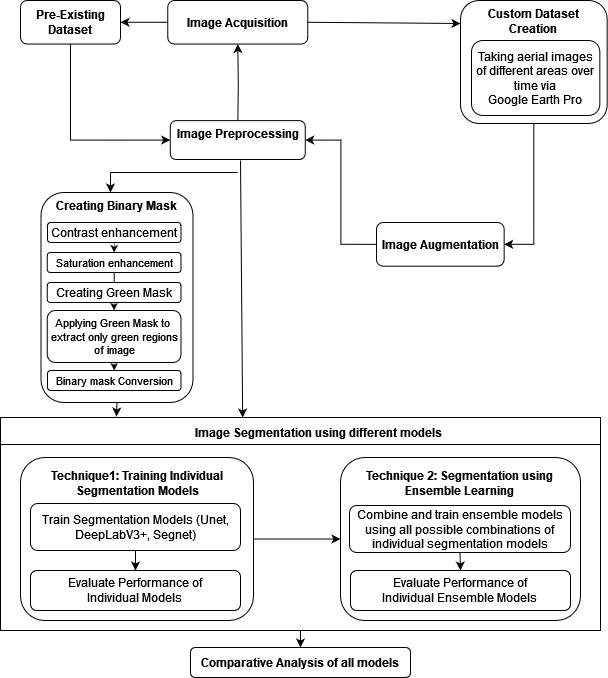
\includegraphics[width=1\textwidth, height=\textwidth,keepaspectratio]{figures/Detection_Methodology.drawio.png}
% \vspace{-25mm}
\caption{Methodology Framework for Detection}
\label{fig:methodology1}
\end{figure}

\begin{figure}
\centering
% \vspace{-30mm}
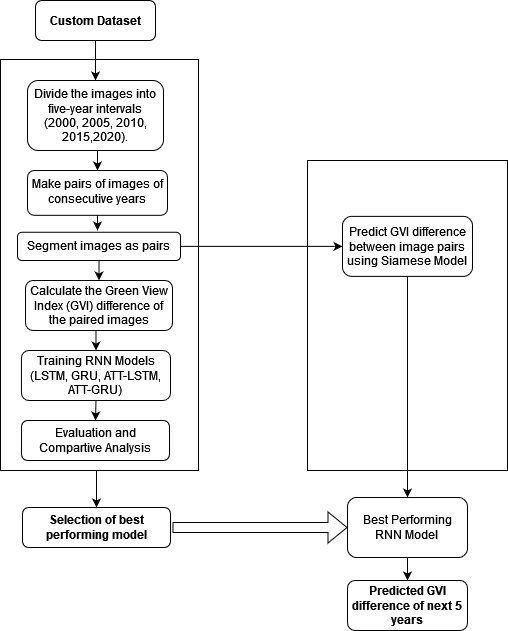
\includegraphics[width=1\textwidth, height=\textwidth,keepaspectratio]{figures/Methodology-prediction.drawio(3).png}
% \vspace{-25mm}
\caption{Methodology Framework for Prediction}
\label{figures/pred_method.png}
\end{figure}


%amrin
\section{Data Acquisition}
The acquisition of required image data was the first focus of this research. Two primary data sets have been utilized to achieve this - a pre-existing data set from Kaggle \shortcite{datasetlink} and a custom data set. The pre-existing data set consisted of 5108 aerial forest images, while the custom data set was created from aerial images of different locations %, captured over a 20-year period 
using Google Earth Pro. The custom data set consists of data from different types of locations such as forest locations, residential locations, and parks from urban locations. To ensure uniformity, all images from both the Kaggle data set and the custom data set are resized to a standardized dimension of 256x256. By resizing the images to an identical size, potential disparities in dimensions are eliminated. 
\subsection{ Kaggle Dataset}
The "Forest Aerial Images for Segmentation" dataset from Kaggle was used. The dataset was obtained from the Land Cover Classification Track in DeepGlobe Challenge \shortcite{demir2018deepglobe}. This dataset contains aerial images of locations with different coverage of land. It also has a variety of barren land and water bodies.  It contained 5108 aerial forest images with dimensions of 256x256. Some example images from the Kaggle dataset are given below in Figure \ref{kaggledataset}. It is visible from the images that the dataset contains a diverse range of land and green coverage and also includes water bodies of different depths and sizes.
\begin{figure}[!htbp]
\centering
 
    \begin{subfigure}[t]{0.15\textwidth}
        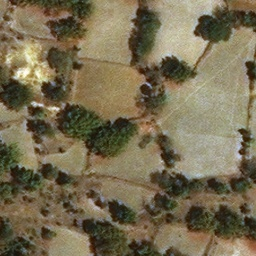
\includegraphics[width=\linewidth]{figures/kaggle (1).jpg}
        %\caption{Image from Forest dataset}
    \end{subfigure}
    \hfill
    \begin{subfigure}[t]{0.15\textwidth}
        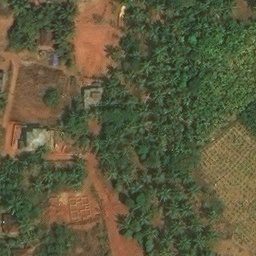
\includegraphics[width=\linewidth]{figures/kaggle (2).jpg}
        %\caption{Image from Residence dataset}
    \end{subfigure}
    \hfill
    \begin{subfigure}[t]{0.15\textwidth}
        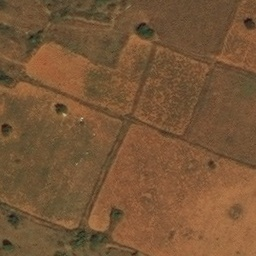
\includegraphics[width=\linewidth]{figures/kaggle (3).jpg}
        %\caption{Image from Park dataset}
    \end{subfigure}
    \begin{subfigure}[t]{0.15\textwidth}
        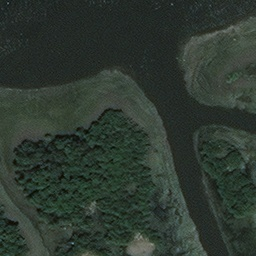
\includegraphics[width=\linewidth]{figures/kaggle (4).jpg}
        %\caption{Image from Forest dataset}
    \end{subfigure} 
    \hfill
    \begin{subfigure}[t]{0.15\textwidth}
        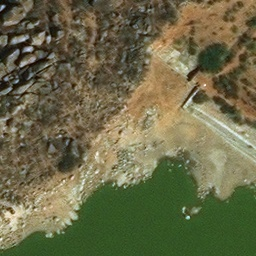
\includegraphics[width=\linewidth]{figures/kaggle (5).jpg}
       %\caption{Image from Residence dataset}
    \end{subfigure}
    \hfill
    \begin{subfigure}[t]{0.15\textwidth}
    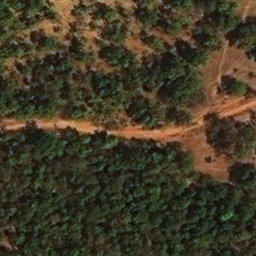
\includegraphics[width=\linewidth]{figures/kaggle (6).jpg}
       % \caption{Image from Park dataset}
    \end{subfigure}
    \caption{Sample Images from Kaggle dataset}
    \label{kaggledataset}
   
\end{figure}




\subsection{Custom Dataset}
 The custom data set was created from aerial images of different locations, captured over 20 years, from 2000 to 2020,
using Google Earth Pro. After enabling historical imagery on Google Earth Pro, a slider is visible showing which years of images are available for the chosen location. Next, the slider is moved to the desired year and month (2000, 2005, 2010, 2015 and 2020). Notably, it was also attempted to maintain consistency in the month chosen for each year's set of images for the same location. Additionally, the view was selected to "Satellite" to get aerial imagery. Images were collected from countries like Canada (Vancouver), Australia (New South Wales, Victoria) and Brazil (Sao Paula)
as images for these countries were available for as old as 2000. The custom data set is subdivided into three categories, namely forest locations, residential locations, and parks. Sample images from the custom dataset are shown in Figure \ref{customdatasetimage}
\begin{figure}[ht]
\centering
 
    \begin{subfigure}[t]{0.15\textwidth}
        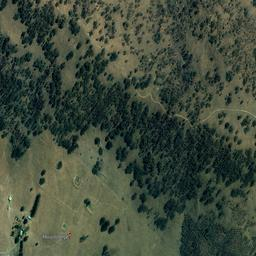
\includegraphics[width=\linewidth]{figures/f1.jpg}
        %\caption{Image from Forest dataset}
    \end{subfigure}
    \hfill
    \begin{subfigure}[t]{0.15\textwidth}
        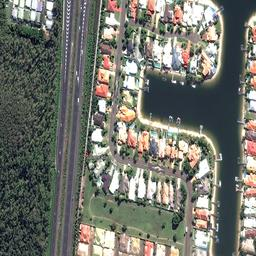
\includegraphics[width=\linewidth]{figures/r3.jpg}
        %\caption{Image from Residence dataset}
    \end{subfigure}
    \hfill
    \begin{subfigure}[t]{0.15\textwidth}
        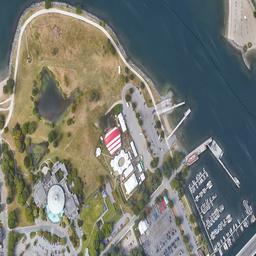
\includegraphics[width=\linewidth]{figures/park1.jpg}
        %\caption{Image from Park dataset}
    \end{subfigure}
    \begin{subfigure}[t]{0.15\textwidth}
        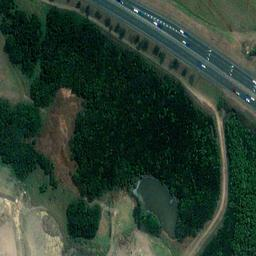
\includegraphics[width=\linewidth]{figures/f2.jpg}
        %\caption{Image from Forest dataset}
    \end{subfigure} 
    \hfill
    \begin{subfigure}[t]{0.15\textwidth}
        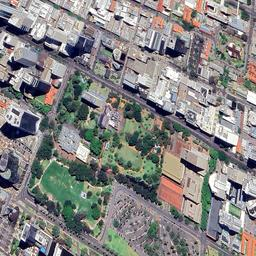
\includegraphics[width=\linewidth]{figures/r2.jpg}
       %\caption{Image from Residence dataset}
    \end{subfigure}
    \hfill
    \begin{subfigure}[t]{0.15\textwidth}
    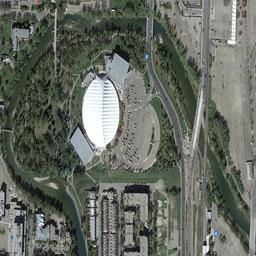
\includegraphics[width=\linewidth]{figures/park2.jpg}
       % \caption{Image from Park dataset}
    \end{subfigure}
    \caption{Sample Images from Categories of Custom Dataset}
    \label{customdatasetimage}
   
\end{figure}



%\section{Image Preprocessing}
%\subsection{Kaggle Dataset}
%\subsection{Custom Dataset}



\subsubsection{Image Augmentation}
Several augmentation techniques that are specific to the images in the custom dataset are used to the data set to keep enhancing it. These methods include a wide range of geometric manipulations, including rotation, shifting, and flipping. For example, an image has been rotated 90 degrees clockwise, counter-clockwise, shifted in different positions, a few were flipped, etc. By using these various augmentation combination, the main motive is to increase the volume and diversity of the training data by applying various changes to the images. This augmentation method improves the segmentation models by emphasizing a deeper understanding of the various ways that green spaces can appear. As a result, the models have more stability, which makes it easier to identify and distinguish green locations in the images. A breakdown of the custom dataset is shown below in Table \ref{customdataset}

 \begin{table*}[h]
\centering
\caption{Breakdown of the Custom Dataset}
\label{customdataset} % Use a different label to avoid conflicts
\small % Reduce font size
%\def\arraystretch{0.9}
%\resizebox{\textwidth}{!}{234
\begin{tabular}{llll}
\hline
SL. No & Category Name & Original Images & After Augmentation  \\
\hline
1 & Forest & 155 & 510 \\
2 & Park & 234  & 563 \\
3 & Residence & 281 &  632\\
\hline
\multicolumn{2}{l}{\textbf{Grand total}} & \textbf{} & \textbf{1,705} \\
\hline
\end{tabular}
}
\end{table*}





%Pinky
\begin{comment}
    \section{Image Preprocessing}
\subsection{ Kaggle Dataset
}  Two methods from the Keras library, a high-level neural networks API built on top of Tensorflow, are utilized for
image preprocessing.
\textbf{ImageDataGenerator-}
 It is used to enhance and prepare visual data for neural network training and testing. Transformations of a picture can be specified, including scaling, rotation, shearing, and normalization, among others.
 \textbf{preprocess\_input-}
 It is utilized to prepare input photos for the CNN model. When the CNN model was trained on the ImageNet 
dataset, the same mean subtraction and scaling were applied as in this function. This preprocessing of the input data
 ensures that the model can extract useful characteristics from the photos.
\subsection{Prepared Dataset}

In the Kaggle dataset, there were no low-quality images, so even without image processing, the model would still
 produce superior results. However, in the prepared dataset, numerous low-quality images have been added, necessitating 
preprocessing in this case. In order to improve image quality, such as by removing noise and artifacts, image 
preprocessing is required. In general, picture preprocessing helps to ensure that the data is in a consistent format and
 improves the data quality, which results in better performance of machine learning models. For picture preparation, two
 techniques from the Keras library, a high-level neural networks API built on top of Tensorflow, are used. The  \textbf{ ImageDataGenerator}  class provides a convenient way to generate batches of image data with real-time data augmentation.
 It supports a wide range of image preprocessing functions, including scaling, rotation, shearing, normalization, and 
data augmentation, among others.
\ref{fig:Preprocessed_Image}.

\begin{figure} [H]
\centering
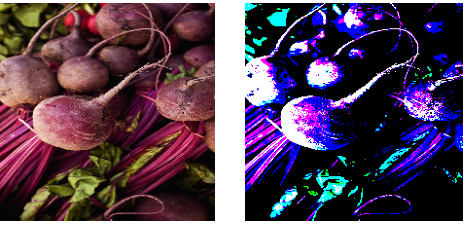
\includegraphics[width=150mm,height=80mm]{figures/Preprocessed_Image.png}
\caption{Preprocessed Image}
\label{fig:Preprocessed_Image}
\end{figure}

\end{comment}

\subsection{Binary Mask Generation}
To create a binary mask highlighting green vegetation in an image, several steps were undertaken. Initially, the image's contrast is enhanced to improve visual clarity, followed by saturation enhancement to amplify color information. Subsequently, a green mask is generated to isolate spaces with green hues. This mask is then applied to the original image, extracting only the green regions while removing non-green elements. Finally, the extracted green regions are converted into a binary mask, representing vegetation as white and non-vegetation as black pixels. This simplified process enables the isolation and identification of green vegetation within the image, facilitating further analysis or applications such as vegetation mapping and environmental monitoring.

\subsection{Splitting into Train and Test Data}
Splitting into train and test sets ensures that the models are trained on sufficient data while also allowing their performance to be assessed on unseen data.
Both datasets is separately split into train and test sets with a ratio of 80\% and 20\% respectively. The test dataset with 20\% of the images serves as a holdout set to assess the model's performance on unseen data.
\section{Green Space Detection} 
In order to predict the green space of a location, it is first required to segment the green space from the images. Several segmentation models were explored which have been discussed further and as shown earlier in Figure \ref{fig:methodology1}, two techniques were used.
This section describes the approaches applied to detect green space from satellite images. 
\subsection{Model Selection for Detection }
This section discusses the segmentation models explored to segment green space from satellite images. 
\subsubsection{U-Net}
Figure \ref{unet_archi} potrays the architecture of U-Net used in this thesis work. The architecture of this model consists of an Input Layer, Contracting Path (encoder), Bottlenck, Expansive Path (decoder) and an Output Layer. In the contracting path, Convolutional blocks were used with increasing filter sizes and depths. Each convolutional block consisted of two 3x3 convolutional layers with ReLU activation and kernel initialization. MaxPooling2D was applied after the first convolutional layer in each block. Dropout layers were added after the first convolutional layer in each block for regularization. Additionally, the number of filters were doubled with each contracting block. In the bottleneck layer, a 3x3 convolutional block was used with dropout. In the Expansive Path, transposed convolutional layers with decreasing filter sizes and depths were used.
Each convolutional block was mapped with the corresponding contracting path
Similar to the contracting path, convolutional layers with ReLU activation and kernel initialization were used along with dropout layers. The output layer contained a sigmoid activation function for binary image segmentation. Adam optimizer was used and Binary cross-entropy loss was used for binary image segmentation.


\begin{figure}[]
    \centering
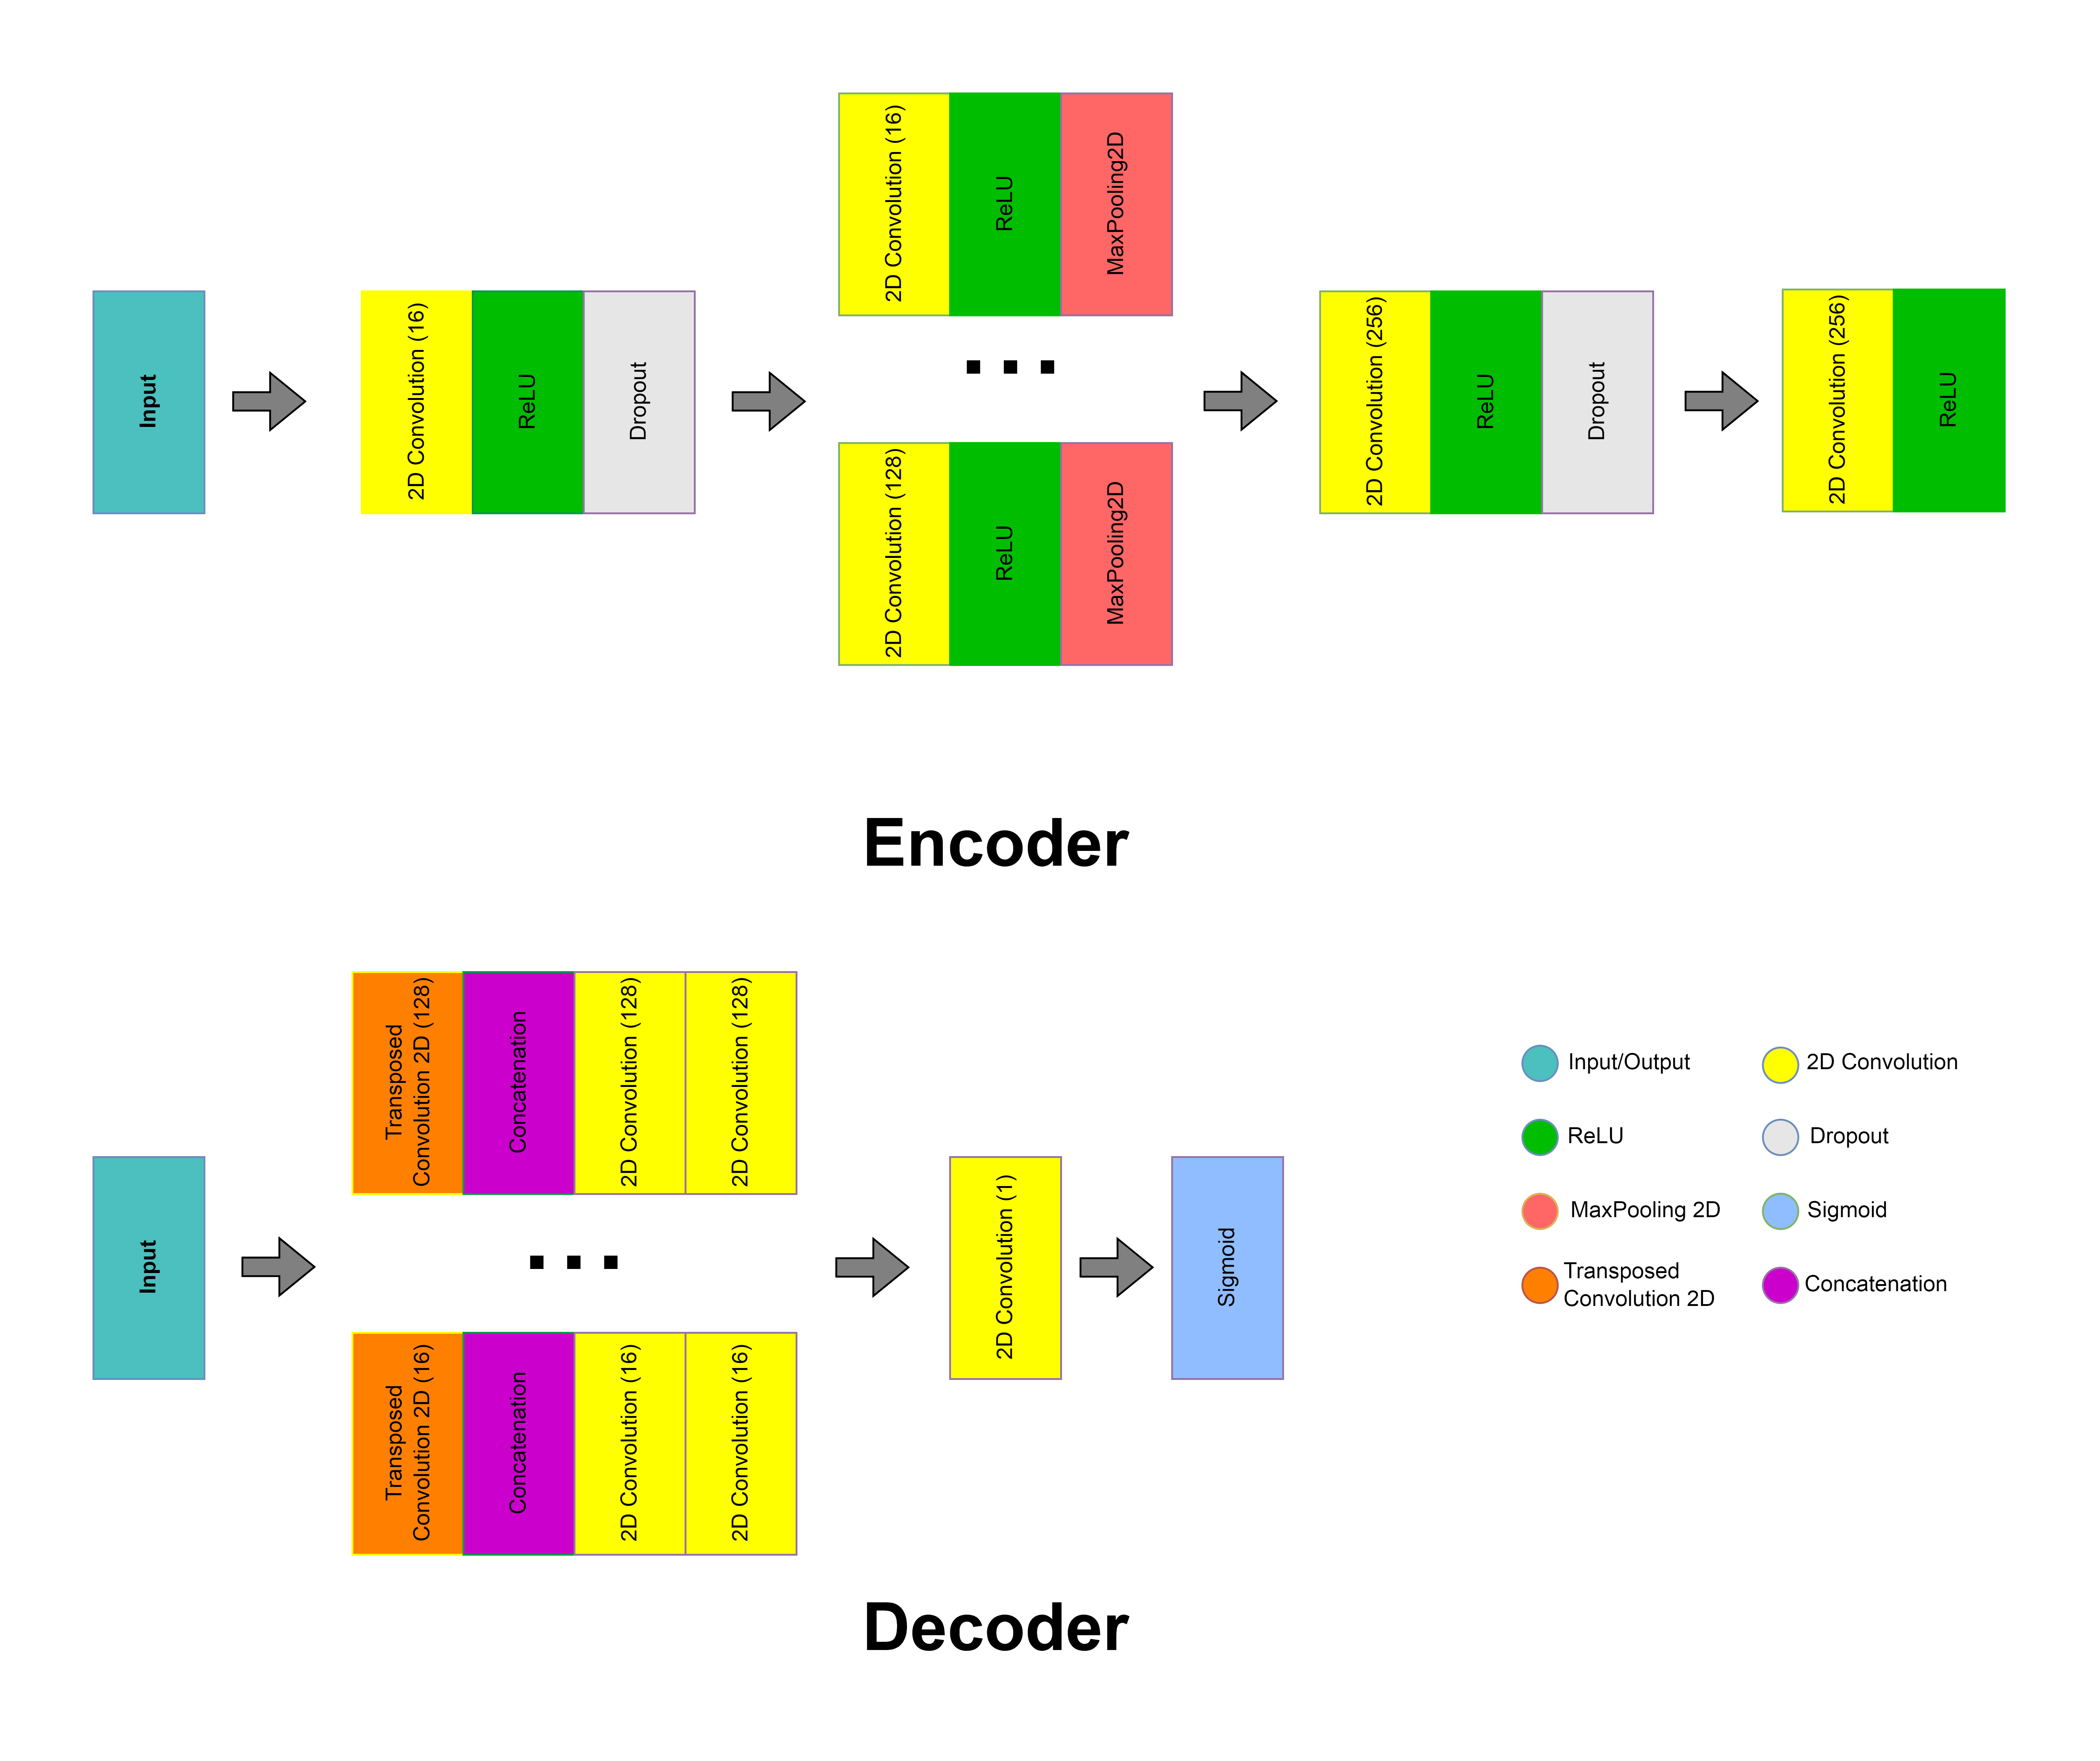
\includegraphics[width=\textwidth]{Unet.png}
    \caption{U-Net Model Architecture}
    \label{unet_archi}
\end{figure}

\subsubsection{SegNet}
SegNet is a convolutional neural network (CNN) architecture designed for semantic segmentation tasks. It consists of an Input Layer, Encoding Layers, Fully Connected (Dense) Layers, Decoding Layer, and an Output Layer. The encoding layer contained several convolutional layers with batch normalization and ReLU activation. Additionally, MaxPooling2D layers were used for downsampling and the number of filters increased deeper into the network. After the encoding layers, two fully connected (dense) layers were added with ReLU activation (1024 units each). In contrast to encoding, the decoding layer consisted of upsampling, and layers were added to perform deconvolution, batch normalization, and ReLU activation was also applied. Additionally, the number of filters decreases in the decoding layers. Finally, the output layer contains one filter and a sigmoid activation function. In this architecture, adam optimizer was used with an initial learning rate of 0.001. The specific architecture used in this thesis work has been displayed in Figure \ref{Segnet_archi}.


\begin{figure}[H]
    \centering
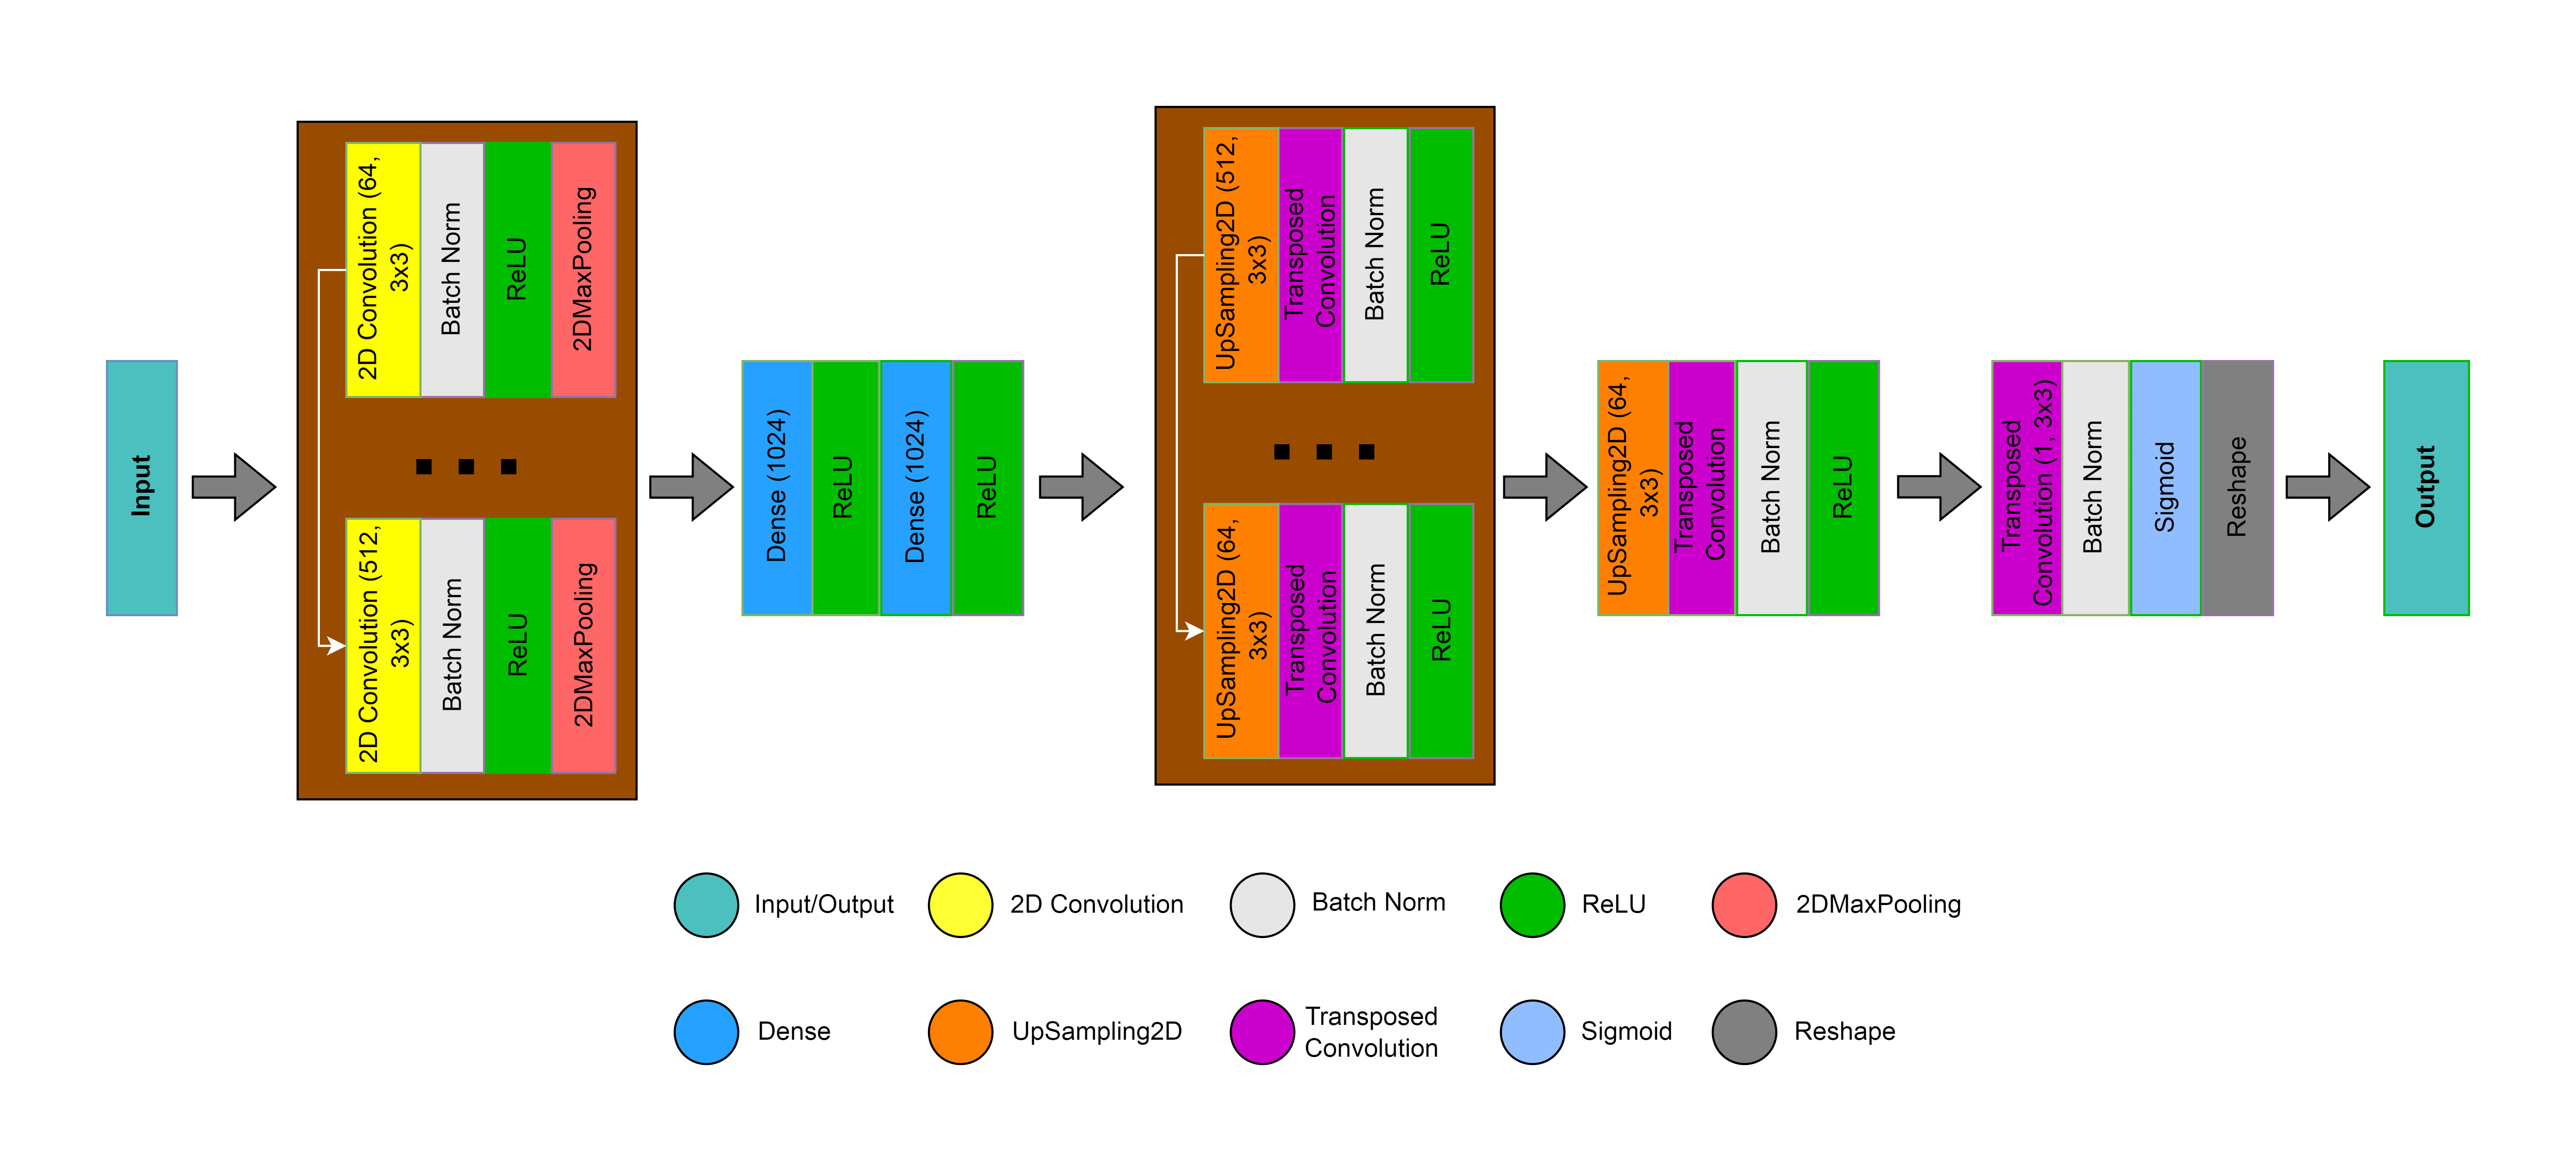
\includegraphics[width=\textwidth]{Segnet(1).png}
    \caption{SegNet Model Architecture}
    \label{Segnet_archi}
\end{figure}

\subsubsection{DeepLabV3Plus}
As shown below in Figure \ref{Deeplabv3_archi}, DLV3Plus utilizes a ResNet50 backbone, a well-established deep learning architecture, to extract features from input images. Additionally, an Atrous Spatial Pyramid Pooling (ASPP) module is employed to capture contextual information at multiple scales, aiding in understanding objects of different sizes within an image. In the research, the model has been optimized using the Adam optimizer with a learning rate of \(1 \times 10^{-3}\) and binary cross-entropy loss, a common choice for binary classification tasks. Accuracy is monitored as a metric during training to evaluate the model's performance. This configuration ensures that the DLV3Plus model is skilled at accurately segmenting objects in images, contributing significantly to the research goals.

\begin{figure}[H]
    \centering
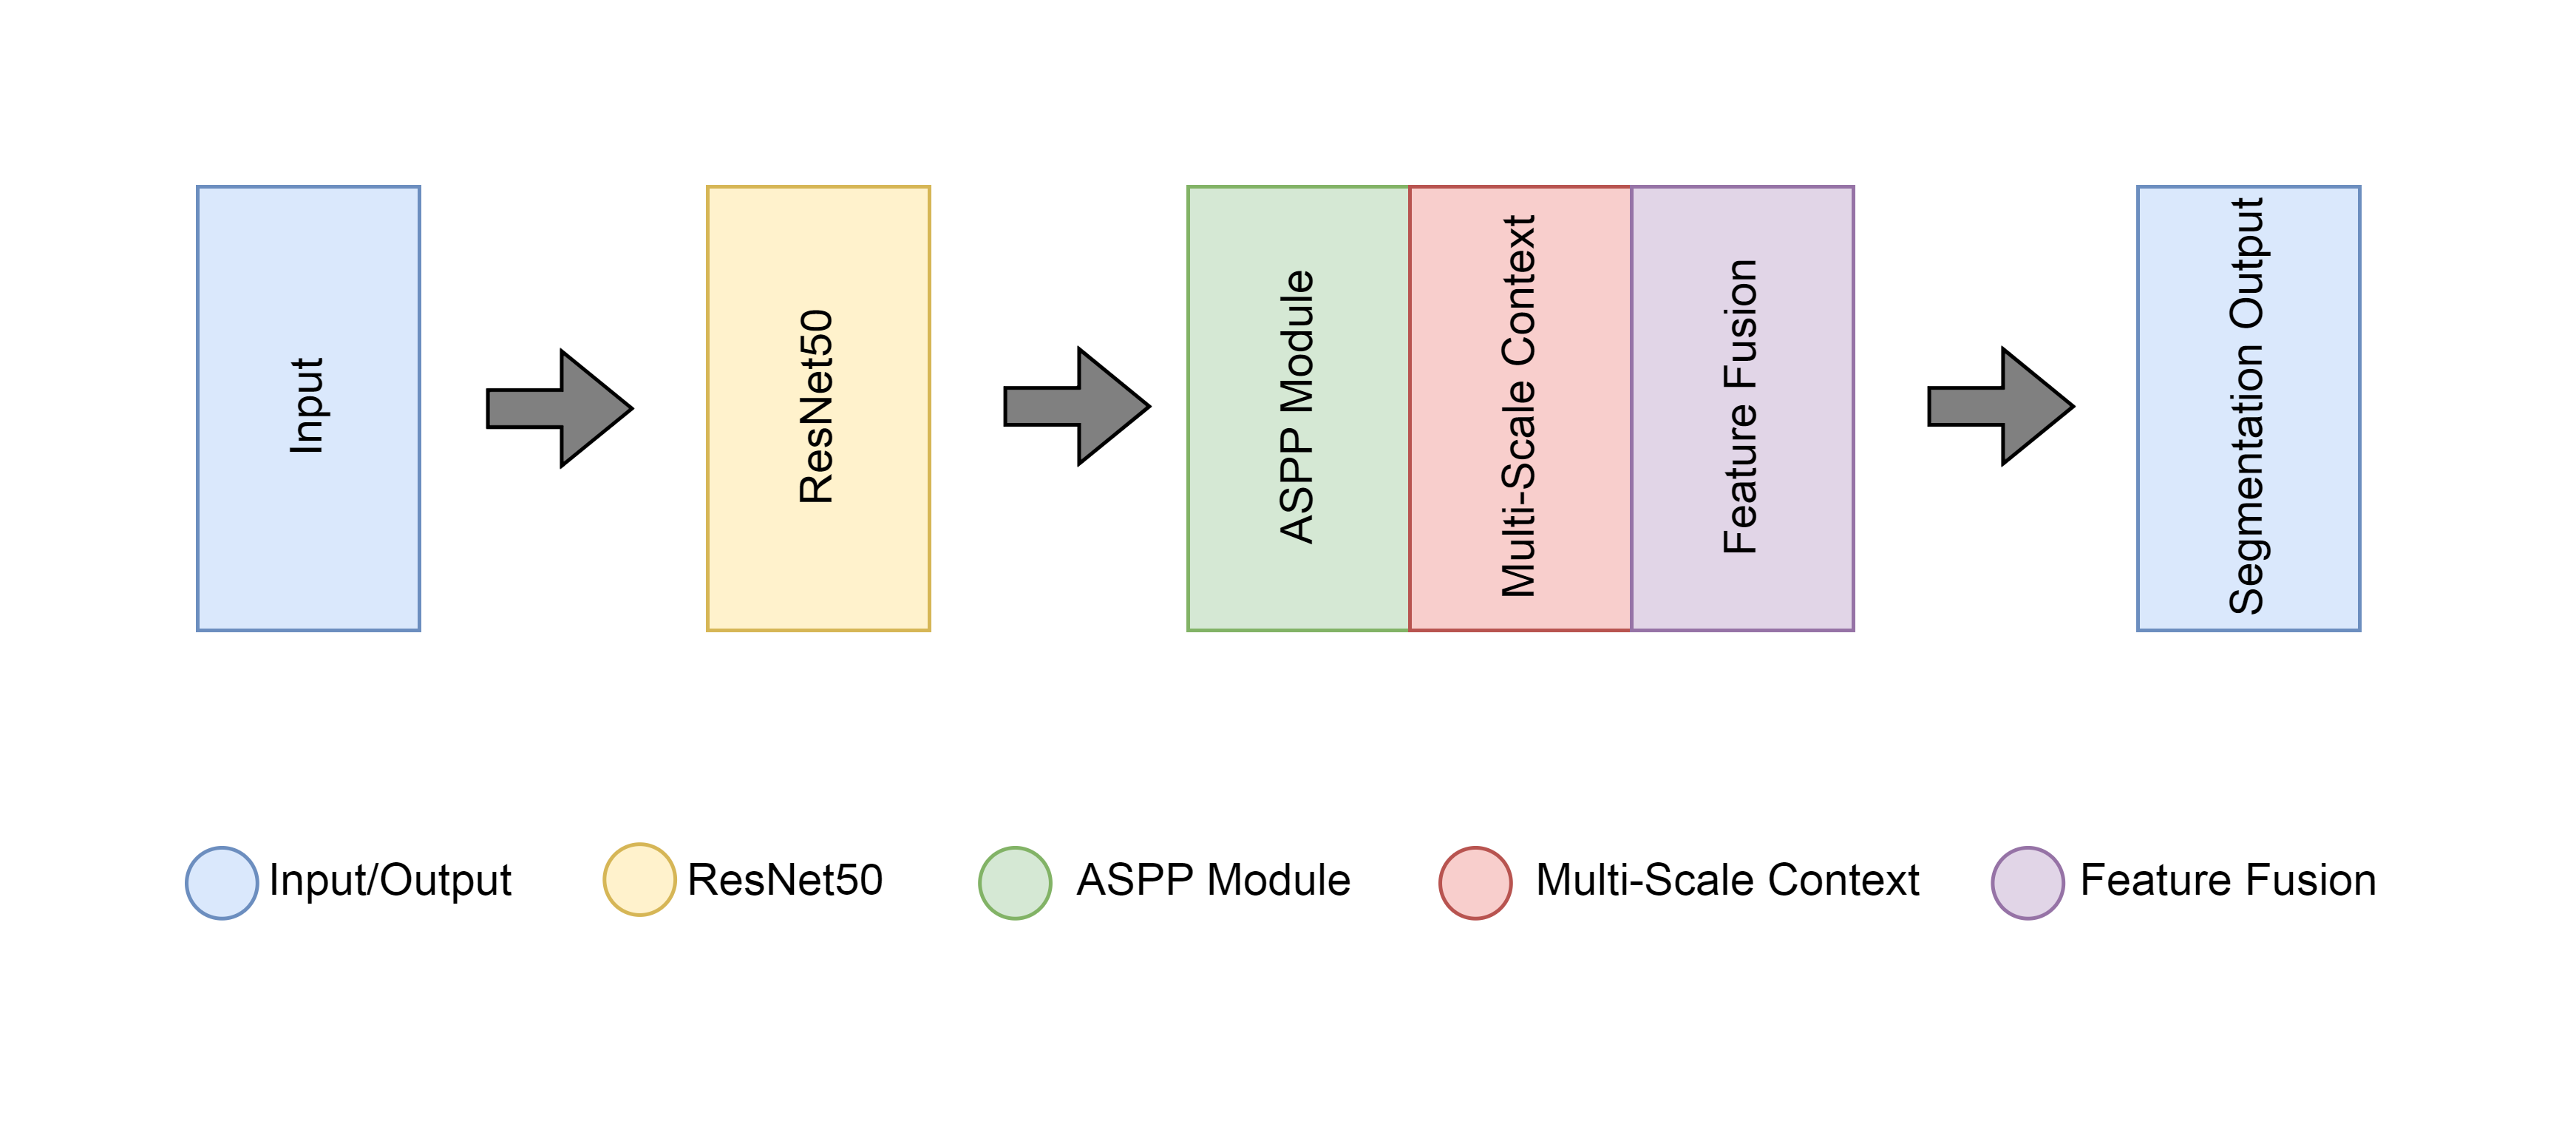
\includegraphics[width=\textwidth]{Deeplav3.png}
    \caption{DeepLabV3plus Model Architecture}
    \label{Deeplabv3_archi}
\end{figure}

.

\subsection{ Technique 1: Training Different Segmentation Models}
Both the pre-processed data set is fed into three different segmentation models: SegNet, UNet, and DeepLabV3+, along with the matching binary masks. The models were chosen for their established success in image segmentation tasks.  %\textcolor{red}{add something saying why these 3 models were chosen.}  
SegNet efficiently handles high-resolution images, UNet demonstrates adaptability across diverse data types, and DeepLabV3+ has a powerful architecture designed for semantic segmentation. This ensures a thorough analysis of green space distribution in designated locations, enhancing the research's reliability. A thorough analysis of the distribution and composition of green spaces in the designated locations is made possible by the meticulous training of each model to precisely identify and segment green locations within the aerial images. The models were trained using both the pre-existing data set and the custom data set separately to prove the robustness of the models.

\subsection{Technique 2:  Ensemble Learning-Based
Approach
}
With this approach, multiple models are effectively combined to produce a single segmentation system. With the help of UNet, Segnet, and DeepLabV3 four ensemble models were created. The combinations of these four models are UNet-Segnet-DeepLabV3,
UNet-Segnet, and UNet-DeepLabV3, and Segnet-DeepLabV3 respectively which is shown in Figure \ref{model2}. The identical method used for training in technique 1 was also used for ensemble learning.
\begin{figure}[H]
        \centering
        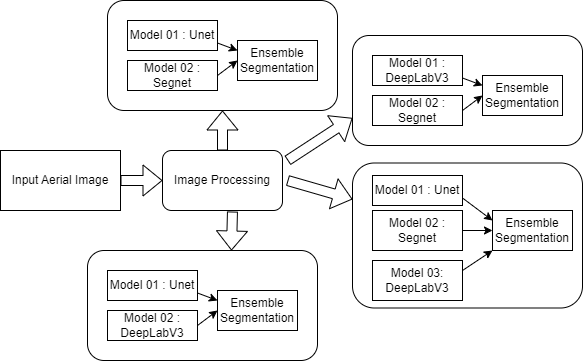
\includegraphics[width=1\textwidth, height=\textwidth,keepaspectratio]{figures/Ensemble Framework.drawio(1).png}
  
\caption{Framework for Ensemble Learning}   
\label{model2}
\end{figure}

\section{Green Space Prediction}
Green View Index (GVI) is a metric used in many research to measure the quantity of green space in a given location. For this reason, it has been chosen as the medium to measure the future amount of green space. In this research, binary segmented images have been used where 0 represents green space and 1 represents non-green space. Hence, based on the work by \shortciteA{yang2009can} and \shortciteA{li2015assessing}, the formula used by calculating GVI in this research is

\begin{equation}
\text{Green View Index (GVI)} = \frac{\text{Total number of white pixels in image}}{\text{Total pixels in image}}
\label{eq:gvi}
\end{equation}

However, rather than just determining the amount of green space, the focus of this research is to identify changes in green space. Therefore, throughout this research, the GVI difference between 5-year intervals has been employed as the data. The approach used for green space detection is covered in this section. 

\subsection{Image Pairing}
The custom dataset contains images of the same location for a time range of 2000 to 2020, with an interval of five years. Firstly, the images were separated into designated years. Next, the images are made into pairs of consecutive images such as Pair $P_i$ \{$Image_{j}$, $Image_{k}$\} 
where \textit{j} is recorded at an earlier timestamp than \textit{k}. Therefore, for each location, there are four pairs of images:
\begin{itemize}
  \item $Pair_1$: \{$Image_{2000}$, $Image_{2005}$\}
  \item $Pair_2$: \{$Image_{2005}$, $Image_{2010}$\}
  \item $Pair_3$: \{$Image_{2010}$, $Image_{2015}$\}
  \item $Pair_4$: \{$Image_{2015}$, $Image_{2020}$\}
\end{itemize} 
This range of years was selected as it is not possible to calculate the ground truth value of years after 2024. In addition, images prior to 2000 are not easily accessible. Therefore, throughout this experiment, 2015 has been considered the present year and 2020 will be the future year following a five-year gap. The Green View Index (GVI) of each image is calculated and then the difference in the GVI between the paired images is calculated as 
%is 
\begin{equation}
    \Delta\text{GVI} = \text{GVI value of Image}_{k} - \text{GVI value of Image}_{j}
    \label{eq:delta_gvi}
\end{equation}

That means, if the GVI difference comes negative, there has been a decrease in green space and a positive GVI difference indicates an increase in green space over the next 5 years.

Finally, after pairing the images and computing their corresponding GVI differences, a redesigned dataset is produced which contains information about 341 locations. There are four data pairings for every place. Table \ref{datasettable} provides an illustration of how the data are organized.

\begin{longtable}{c c c c}
\caption{Redesigned Custom Dataset with Image Pairings} \label{datasettable} \\
\hline
Pair & Image\textsubscript{j} & Image\textsubscript{k} & $\Delta\text{GVI}_{\text{Pair}_i}$  \\
\hline
\endfirsthead

\multicolumn{4}{c}{{\tablename} \thetable{} -- Continued from previous page} \\
%\hline
\textbf{Pair} & \textbf{Image\textsuperscript{j}} & \textbf{Image\textsuperscript{k}} & \textbf{Delta GVI\textsubscript{Pair}} \\
%\hline
\endhead

$P_1$ & 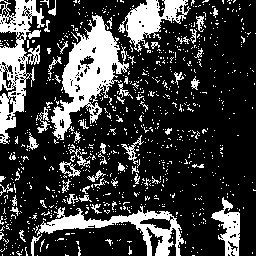
\includegraphics[width=1cm]{figures/pp_augmented_Cyril-2000_mask.jpg} & 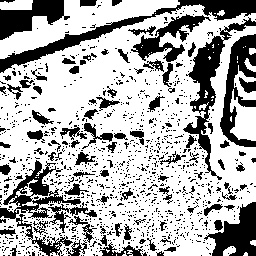
\includegraphics[width=1cm]{figures/pp_augmented_Cyril-2005_mask.jpg} & 30.02\\
%\hline
$P_2$ & 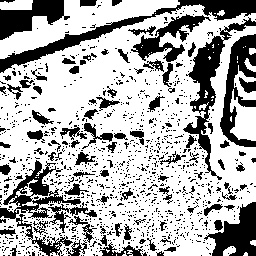
\includegraphics[width=1cm]{figures/pp_augmented_Cyril-2005_mask.jpg} & 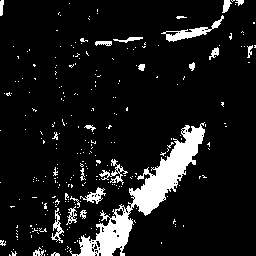
\includegraphics[width=1cm]{figures/pp_augmented_Cyril-2010_mask.jpg} & -39.26 \\
%\hline
$P_3$& 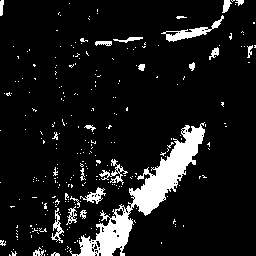
\includegraphics[width=1cm]{figures/pp_augmented_Cyril-2010_mask.jpg} & 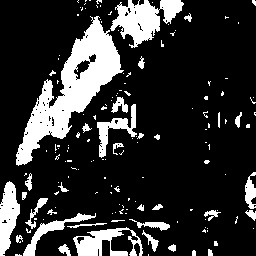
\includegraphics[width=1cm]{figures/pp_augmented_Cyril-2015_mask.jpg} & 7.19\\
%\hline
$P_4$ & 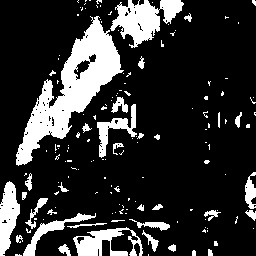
\includegraphics[width=1cm]{figures/pp_augmented_Cyril-2015_mask.jpg} & 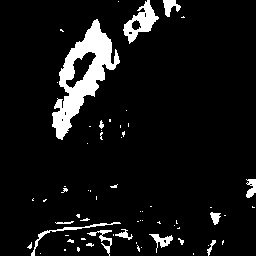
\includegraphics[width=1cm]{figures/pp_augmented_Cyril-2020_mask.jpg} & -8.73 \\
\hline

\end{longtable}


\subsection{Model Selection for Prediction}



Recurrent Neural Network (RNN) models are capable of remembering information learned from prior input while generating outputs. Therefore, they are instrumental in sequential or time series data where each data represents a point in time. RNN models have two types of architecture - Long Short-Term Memory (LSTM) and Gated Recurrent Unit (GRU). Moreover, adding attention mechanisms to the architectures has proven to show better results \cite{RNN1,RNN2}. Therefore, initially, four models have been used to predict the GVI difference over the next 5 years. The selected models have been elaborated further. The results of the models were compared and finally, the best-performing model has been selected for the proposed architecture. In this research, the GVI difference between the years 2000 to 2015 has been utilized to predict the GVI difference in the next 5 years (2015 to 2020).
From the custom dataset, the GVI difference values for $Pair_1$,$Pair_2$ and $Pair_3$ are used as the feature variables and the GVI difference of $Pair_4$ has been used as the target variable. Each pair represents a different point in time. In total, the dataset has information of 341 locations. The RNN models have been then trained on this data.


% The data is split into train data of  80\% and test data of 20\% respectively. All the trained models were evaluated on the testing data. 
% Mean Absolute Error (MAE), Mean Squared Error (MSE), and Root Mean Squared Error (RMSE) were calculated to evaluate the model's performance. All the metrics have been described earlier in Chapter 2.


\subsubsection{Long Short-Term Memory (LSTM)}
The architecture used in this research consists of two LSTM layers with 50 units each, followed by a dense layer with a single output neuron for GVI difference prediction. The model was compiled with separate loss functions for mean squared error (MSE) and mean absolute error (MAE), both optimized using the Adam optimizer. 
%The training was performed for 100 epochs with a batch size of 16.
\subsubsection{Attention Long Short-Term Memory (ATT-LSTM)}
The same LSTM model architecture was applied with an additional custom attention layer to add an attention mechanism. The attention mechanism was employed to give different weights to different parts of the input sequence, emphasizing important information during the learning process. The attention mechanism utilizes trainable weights to compute attention scores for each time step in the LSTM output sequence. The attention scores are applied to the LSTM output sequence, giving higher importance to certain time steps. %However, unlike, basic LSTM, attention-LSTM was trained on epoch 100 with a batch size of 4 as higher batch sizes showed signs of overfitting.
\subsubsection{Gated Recurrent Unit (GRU)}
Similar to LSTM, the input layer of the Gated Recurrent Unit (GRU) model starts with 50 units and a "return sequences" parameter returns the full sequence of outputs for each input sequence. The second layer also consists of 50 units and a dense layer with a single output neuron was added for the GVI difference prediction.
%The model was trained on the training data with 100 epochs and batch size 16 and compiled using the mean squared error loss function and the Adam optimizer. 

\subsubsection{Attention Gated Recurrent Unit (ATT-GRU)}
The exact architecture of the GRU model was used in addition to a custom attention layer. This layer acts as an attention mechanism. In this layer, parameters (weights and biases) are learned during training. The attention mechanism computes attention scores for each time step, focusing relevant information in the input sequence.

\subsection{Siamese Neural Network Model}

\begin{figure}[H]
    \centering
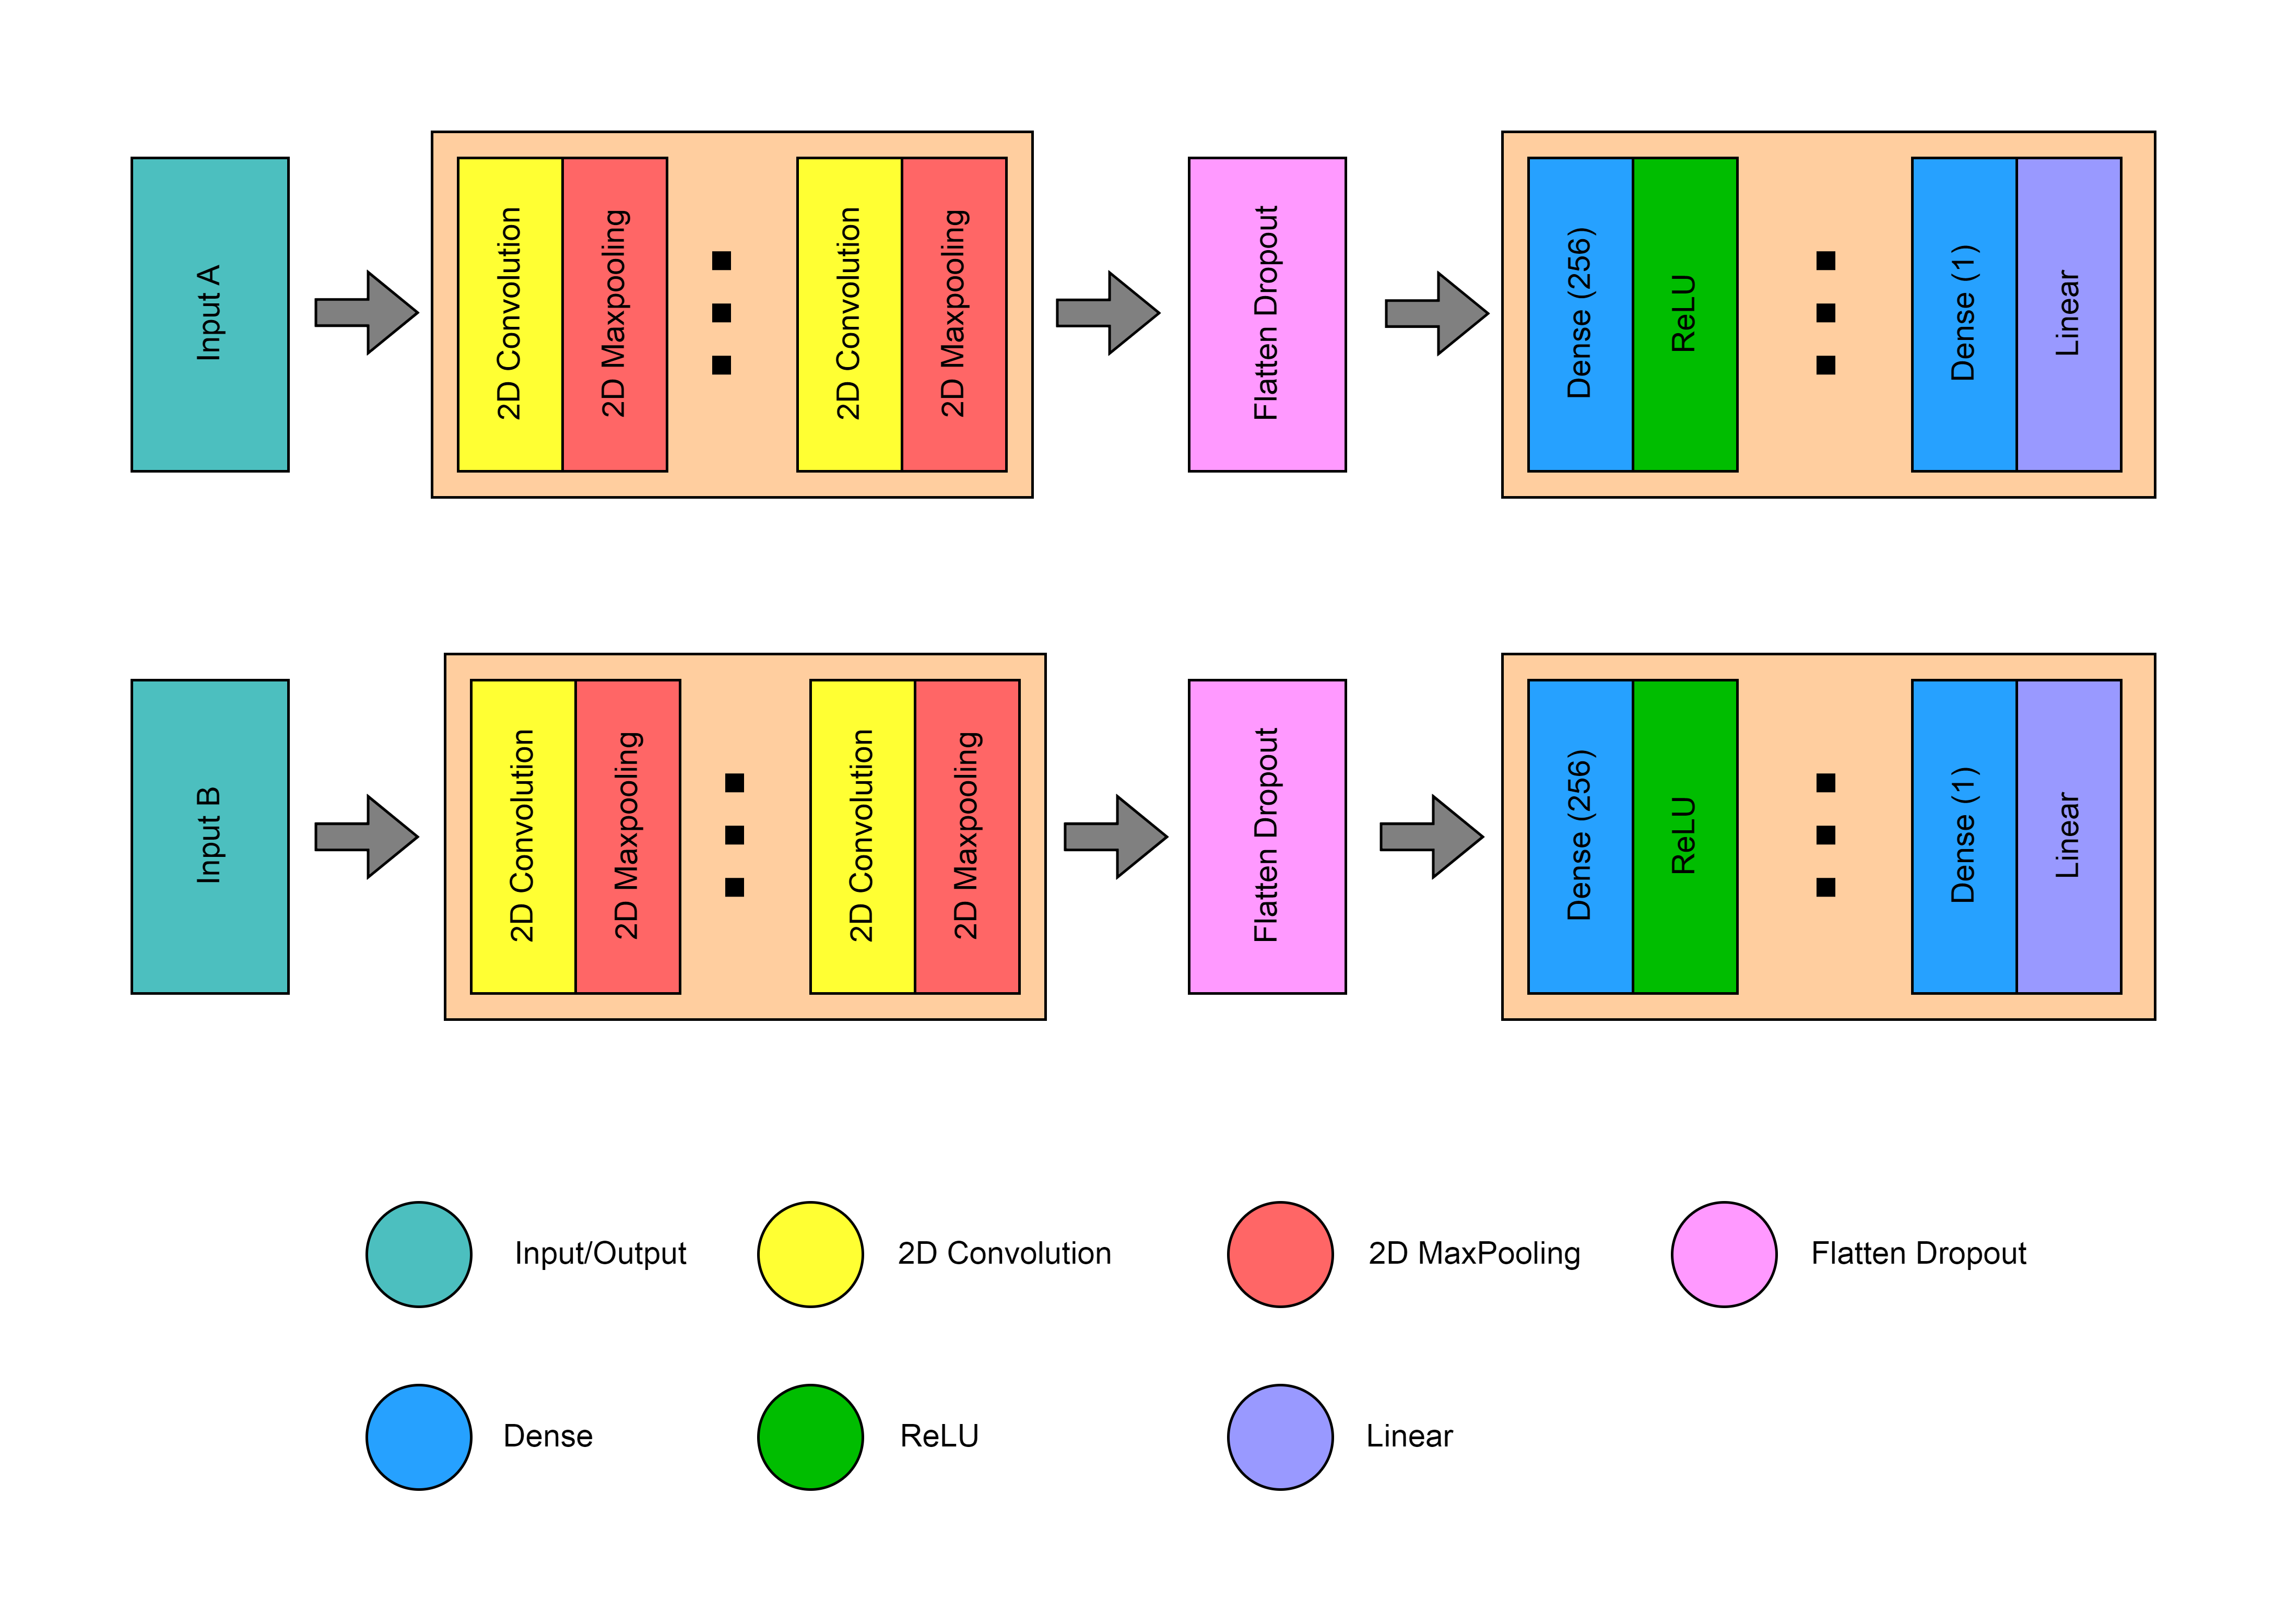
\includegraphics[width=\textwidth]{Siamese.png}
    \caption{Siamese Neural Network Model Architecture}
    \label{siamese_archi}
\end{figure}
Siamese Neural Network is a reliable and robust architecture for detecting similarity between images and has been applied in various fields, from person identification \shortcite{siamese1} to detecting change in land \shortcite{siamese2}. In this research, 4 individual siamese models were trained with segmented images of a specific pair {$Pair_1$,$Pair_2$,$Pair_3$,\\$Pair_4$}. The segmented images used have been generated earlier in the green space detection phase of this research. So, a pair for the segmented image was given as the feature variables and the target variable was the GVI difference between the two images.

%To evaluate the model's performance, test data (20\% of the dataset) was used to make predictions and the results were compared with ground truth values to calculate the mean square error, mean absolute error, and root mean square error of the model. The methodology followed is illustrated in \ref{}.













As shown in Figure \ref{siamese_archi}, the Siamese model architecture used in this research consisted of shared convolutional layers followed by separate branches for each input image. The branches had fully connected layers, and the final output was obtained by concatenating the outputs of these branches and passing through a regression output layer. The shared convolutional layer was made up of three layers containing 32,64 and 123 filters respectively of kernel size (3,3) along with ReLu activation function and MaxPooling layer. The applied architecture also consisted of a dropout layer with a dropout rate of 0.5 for regularization. The separate branches for each input image contained two fully connected layers with 256 units and ReLU activation for each input branch.


\section{Proposed Framework}

\begin{figure} [H]
\centering
% \vspace{-30mm}
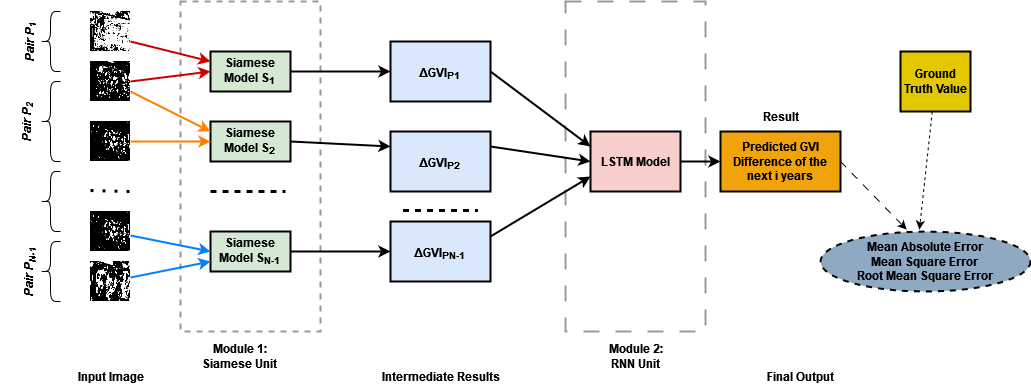
\includegraphics[width=\textwidth, height=\textheight, keepaspectratio]{figures/Methodology-Prediction Framework.drawio.png}
% \vspace{-25mm}
\caption{Proposed Framework for Predicting Change in GVI from Historical Images}
\label{framework}
\end{figure}

The goal of this research is to predict the change in green space of a location in the next 5 years, based on past historical images of the said location. To do so, a two-module framework is proposed, as shown in Figure \ref{framework}. Suppose there are N images of a selected location $\{y_{T}, y_{T+i}, \ldots, y_{T+(n-1)i}$\} where \textit{T} is the earliest year, \textit{N} is the number of images and \textit{i} represents the interval considered (in this research, interval is considered as 5). These images are now made into pairs of non-overlapping consecutive years. So, from N images, there will be a total of N-1 Pairs.





Module 1, which is the Siamese unit, consist of multiple siamese model S = \{$S_1$, $S_2$, ... $S_n-1$\}. Each pair $P_i$ is sent to the i-th siamese model. Siamese model takes segmented image of consecutive years as input and as output, gives a predicted GVI difference between the images. These are the intermediate result of the proposed framework. 
%The formula of the predicted GVI difference  for a Pair $P_i$ \%{$Image_j$, $Image_k$\} is 
%\[ \Delta\text{GVI}_{\text{P}_i} = \text{GVI value of Image}_k - \text{GVI value of Image}_j \]

%where \textit{j} is recorded at an earlier timestamp than \textit{k}. That means, if the GVI difference comes negative, there has been a decrease in green space and a positive GVI difference indicates an increase in green space over the next 5 years. 

In module 2, the RNN unit, the intermediate results achieved from module 1 are concatenated $\{\Delta\text{GVI}_{\text{P}_1\\}, \Delta\text{GVI}_{\text{P}_2}, \ldots,
\Delta\text{GVI}_{\text{P}_{N-1}}\}$ and sent to an LSTM model. Based on the result analysis in Chapter 4, the LSTM model is found to be the best-performing RNN model. LSTM is trained to learn long-term dependencies in sequential data. The model is given a
range of GVI differences with an \textit{i}-year gap (in this case, \textit{i}=5), and based on this data, the final predicted
GVI difference for the next \textit{i} years is achieved.



\begin{comment}
    

For green segmentation, several factors were considered for model selection to ensure optimal performance. 
Searching and recommendation are undoubtedly classification problems. Hence it requires classification algorithms to solve. Convolutional Neural Networks (CNNs) is the type of deep learning model that are designed to process and analyze data with a grid-like topology, such as an image, and are particularly well-suited for image recognition and classification problems. In a CNN, the input image is convoluted with a set of filters to extract features and reduce the dimensionality of the image. The output of this convolution is then passed through a pooling layer, which downsamples the image and reduces the computational load. The process is repeated multiple times to extract higher-level features from the image, and the final layer is a fully connected layer that uses these features for classification. They have been used to achieve state-of-the-art results in a variety of computer vision tasks, including object detection, image segmentation, and image generation. 

Pre-trained CNN models which are large, deep learning models trained on a large dataset for a related task (e.g. image classification) are used for this study through transfer learning technique. Transfer learning is a machine learning technique that involves reusing pre-trained models on new, related tasks. The idea behind transfer learning is that a model that has been trained on a large dataset for a similar task can be used as a starting point for a new task, allowing the model to learn faster and achieve better performance than if it were trained from scratch. It is especially useful when there is a limited amount of labeled data available for a new task, as the pre-trained model provides a good representation of the data that can be fine-tuned for the new task. It has been successfully applied in many domains, such as computer vision and natural language processing. \cite{5_meth} represented the transfer learning architecture as shown in figure \ref{fig:transfer}. Transfer learning works in the following way.

 \begin{itemize}
 \item Pre-trained model: A large, deep learning model is trained on a large dataset for a related task (e.g. image classification).

\item Feature extraction: The pre-trained model is used to extract the features (or representations) of the input data.

\item Fine-tuning: The extracted features are used to train a new, smaller model for the new task. The weights of the pre-trained model may be frozen, or fine-tuned to adapt to the new task.

\item Task-specific output layer: The final, task-specific output layer is added to the model to produce the desired predictions for the new task.
 \end{itemize}
 
\begin{figure} []
\centering
% \vspace{-30mm}
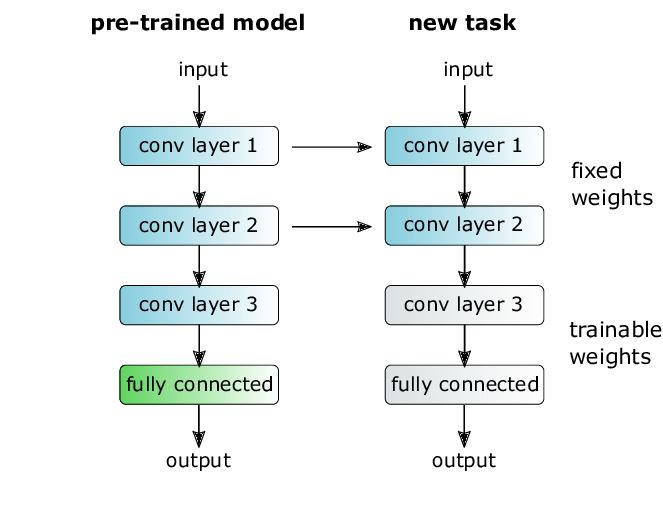
\includegraphics[width=130mm,height=110mm]{figures/transfer.png}
% \vspace{-25mm}
\caption{Schematic View of Transfer Learning}
\label{fig:transfer}
\end{figure}
 

\subsection{ Classification and Category prediction}
Out of many popular CNN algorithms, three seemed to be the perfect fit for the implementation of the classification and category prediction part which are VGG16, ResNET50, and MobileNET.
 These three pre-trained models have been used separately through transfer learning and combined through ensemble learning to find out the combination with the best results. An elaborate description of these models is given below.
\\
\textbf{VGG16:} 

\begin{itemize}
\item Input layer: This layer feeds images into the network. It is merely a placeholder for the given images as it does not have any learnable parameters (weights or biases).
\item Convolutional layer: Input images are processed using a set of small  filters to generate a feature map. The purpose of the feature map is to highlight the most relevant features of the image. Features like edges and corners are to be extracted from the input image. The feature map of the image is generated by performing a dot product between the values in the filters and the corresponding input image values.
\item ReLU layer: In this layer, the feature map acquired from the convolutional layer is processed by applying the ReLU activation function. In this process, negative values are replaced with zeros to prevent the system from getting stuck in a non-convergent state with decreasing accuracy.

\item Pooling layer: This layer works with the feature map generated by the previous ReLU layer to reduce the computational requirements of the network by reducing the spatial size of the map. This reduction is done using down-sampling. Max-pooling is used mostly which selects the maximum value from a set of adjacent pixels. The feature map is divided into a number of non-overlapping regions, and the maximum value is chosen from each region to create the max pooling layer. The resulting down-sampled feature map is then fed into the network's subsequent layer as input.
Now, repeat steps 2-4 multiple times to create multiple convolutional, ReLU, and pooling layers, until the desired number of layers is reached.

\item Fully connected layer: 


The final pooling layer's output is used in this layer to feed a group of densely linked (completely connected) neurons. These neurons make predictions about the input image based on the feature map created by the preceding layers. A prediction for a classification challenge is often produced using this layer. The output of each neuron in the fully connected layer indicates the expected probability for a particular class, and the number of neurons there is equal to the number of classes in the classification task.

\item Softmax layer: This layer creates a probability distribution over the potential classes by applying the softmax activation function to the output of the fully linked layer. The forecast for the input image is then chosen from the class with the highest likelihood.
For classification issues, this layer is frequently utilized in the last layer of a neural network. The fully connected layer and softmax layer are generally combined in the VGG-16 network to produce a prediction for a multi-class classification task.

\end{itemize}

\begin{figure} [H]
\centering
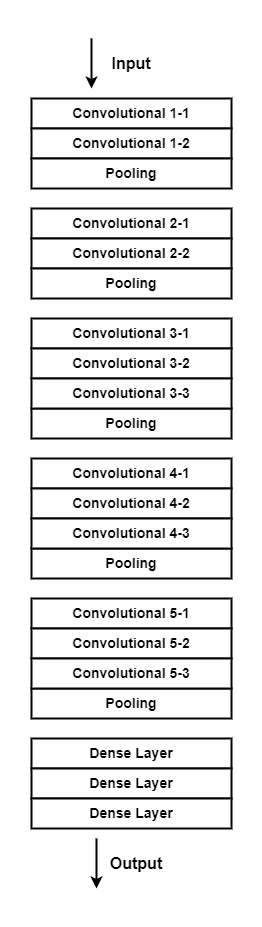
\includegraphics[width=70mm,height=210mm]{figures/VGG16.png}
\caption{VGG-16}
\label{fig:vgg16}
\end{figure}



%naw

\textbf{Resnet50: } %pinky
ResNet50 is a 50-layer deep convolutional neural network (CNN) architecture made up of a number of dense and 
convolutional layers. It was first presented in 2015, and since then, because to its strong performance and reasonably 
lightweight architecture, it has gained popularity for picture classification jobs.The utilization of residual connections, which allows for deeper networks without experiencing the vanishing gradient problem, is the main contribution of ResNet50. The network finds it challenging to learn due to the vanishing gradient problem, which occurs when the gradients in the optimization process get very small. This problem is resolved by residual connections, which enable gradients to directly backpropagate to shallower layers while avoiding particular layers. With over a million photos and 1,000 categories, the ImageNet dataset served as the basis for ResNet50's pre-training. As a result, time and computational resources are saved because the weights of the network have already been modified for the purpose of image classification. The pre-trained model can then be adjusted on fresh data for a particular
 classification task, including object detection, semantic segmentation, or medical imaging.

 ResNet50 is frequently employed for computer vision tasks like facial identification, image categorization, and object recognition. Due to the network's prior learning of valuable characteristics from the ImageNet dataset, it is also a well-liked option for transfer learning, which is the process of applying a network that has already been trained to a new task. ResNet50 has also been applied in a variety of fields, such as robotics, self-driving automobiles,and video categorization.To extract information from an input image, ResNet50 uses a deep convolutional neural network (CNN) architecture with many layers. The primary categories of layers in ResNet50 are briefly described below:
 
\begin{itemize}
\item Convolutional layers:The local features of the input image are extracted using these layers. In order to find edges,
 textures, and other patterns, they apply a number of filters on the image.
\item Pooling layers: The convolutional layers' feature maps produced by these layers have smaller spatial dimensions. By 
subsampling the feature maps, they aid in reducing computational costs and preventing overfitting.
\item Residual blocks: These comprise two or more layers with a residual connection and are the ResNet50 building blocks. The
 gradients can directly backpropagate to shallower layers thanks to the residual connection, which helps solve the 
disappearing gradient issue.


    

    
\item Dense layers: These are fully connected layers that are used to make the final classification. They take the features 
produced by the residual blocks and produce the final output.
\end{itemize}


\begin{figure} [H]
\centering
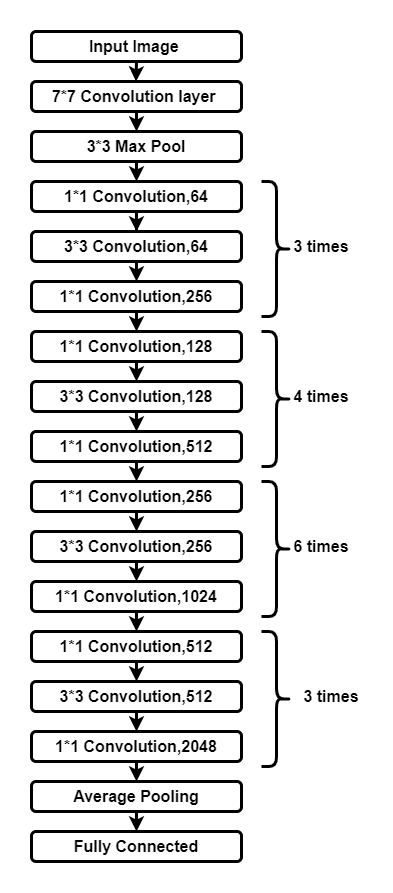
\includegraphics[width=90mm,height=210mm]{figures/ResNet.png}
\caption{ResNet50}
\label{fig:resnet}
\end{figure}


ResNet50 can learn both high-level and low-level characteristics from an input image thanks to the mixture of these
 various sorts of layers, which is essential for effective performance on image classification tasks. ResNet50 also has a
 very deep architecture without encountering the vanishing gradient problem, which is a prevalent difficulty in deep 
neural networks, thanks to the usage of residual connections.
\\
\\
\textbf{MobileNet: } 
MobileNet is a lightweight deep learning model developed by Google, specifically designed for deployment on mobile and embedded devices with limited computational resources. It is a type of Convolutional Neural Network (CNN) that uses depthwise separable convolutions to reduce the number of parameters and computations, making it faster and more efficient compared to traditional CNNs.

In a depthwise separable convolution, the input is first convolved with a set of filters to extract features from the input, and then these features are concatenated and processed by another set of filters to produce the final output. This process reduces the number of parameters and computations compared to traditional convolutions, making it more efficient for deployment on mobile and embedded devices. It uses a series of these depthwise separable convolutions to extract features from the input image, followed by a few fully connected layers to produce the final output. It has been trained on large datasets and can be used for a variety of computer vision tasks, including image classification, object detection, and semantic segmentation. Some of the key layers used in a MobileNet model are as follows.

\begin{itemize}
\item Convolutional layer: The first layer of a MobileNet is a convolutional layer that applies a set of filters to the input image to extract features and reduce the dimensionality of the image.
\item Depthwise separable convolution layer: MobileNet uses a special type of convolution called a depthwise separable convolution, which reduces the number of parameters and computations compared to traditional convolutions. In this layer, the input is first convolved with a set of filters to extract features, and then these features are concatenated and processed by another set of filters to produce the final output.

\item Pointwise Convolution layer: The Pointwise Convolution layer performs 1x1 convolutions to map the input features to a desired number of output channels.

\item Pooling layer: A pooling layer downsamples the image and reduces the computational load, making the model more efficient. In MobileNet, a global average pooling layer is often used as the final pooling layer to produce a fixed-length output vector.

\item Fully connected layer: The final layer of a MobileNet is a fully connected layer that uses the extracted features to make a prediction.
\end{itemize}

\begin{figure} [H]
\centering
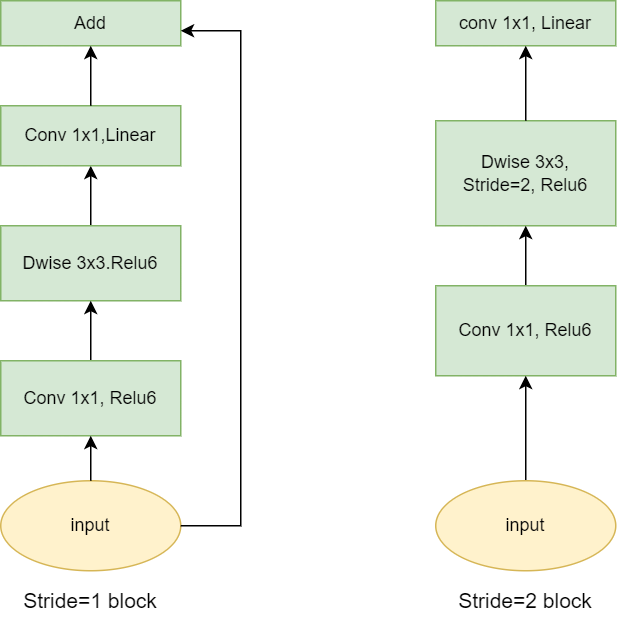
\includegraphics[width=90mm,height=210mm]{figures/mobilenet.png}
\caption{MobileNet}
\label{fig:mobilenet}
\end{figure}

These layers are repeated multiple times in a MobileNet model to extract higher-level features from the input image and produce a final prediction. The exact number and type of layers used can vary depending on the task and the desired accuracy, but these are the key components of a typical MobileNet model.

For the classification part MobileNetV2 model is used which is an updated version of the MobileNet architecture. It introduces several changes to the original MobileNet architecture, including the use of inverted residual blocks, linear bottlenecks, and a low-resolution shortcut to improve performance [\cite{1_meth}]. The inverted residual block allows the model to learn more complex representations, while the linear bottlenecks and low-resolution shortcut help reduce computation and improve efficiency. The key layers of MobileNetV2 are somewhat different from MobileNet which are discussed below.


\begin{itemize}
\item Inverted residual block: The core building block of a MobileNetV2 is an inverted residual block, which consists of a depthwise separable convolution, a pointwise convolution, and a residual connection. The depthwise separable convolution extracts features from the input, and the pointwise convolution maps these features to the desired number of output channels. The residual connection allows the network to learn residuals, or the differences between the input and output of each block, to improve performance.

\item Depthwise separable convolution layer: MobileNetV2 uses depthwise separable convolutions to reduce the number of parameters and computations compared to traditional convolutions. In this layer, the input is first convolved with a set of filters to extract features, and then these features are concatenated and processed by another set of filters to produce the final output.

\item Pointwise Convolution layer: The Pointwise Convolution layer performs 1x1 convolutions to map the input features to a desired number of output channels.

\item Linear bottleneck: A linear bottleneck layer reduces the number of parameters and computations in the model, making it more efficient.

\item Low-resolution shortcut: A low-resolution shortcut helps the model capture information from different scales by bypassing the inverted residual blocks and concatenating the output of these blocks with the output of the shortcut.

\item Global average pooling layer: The final layer of a MobileNetV2 is a global average pooling layer, which downsamples the image and reduces the computational load, making the model more efficient. It also produces a fixed-length output vector.
\end{itemize}


The architecture of MobileNetV2 is designed to balance accuracy and efficiency, making it well-suited for deployment on mobile and embedded devices. It contains the initial fully convolution layer with 32 filters, followed by 19 residual bottleneck layers [\cite{2_meth}]. [\cite{2_meth}] represented the MobileNetV2 model as shown in figure \ref{fig:mobilenet}.


% \begin{figure} [H]
% \centering
% 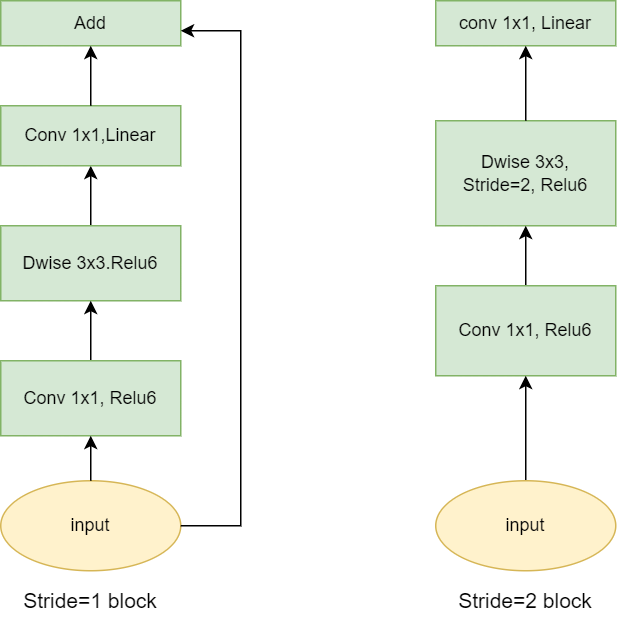
\includegraphics[width=90mm,height=210mm]{figures/mobilenet.png}
% \caption{MobileNet}
% \label{fig:mobilenet}
% \end{figure}

%naw
\section{Green Space Prediction}
\begin{comment}
    

To determine image similarity and product recommendations, there are many techniques available out of which two were chosen alongside the three previous techniques used in classification and category prediction.

\textbf{KNN:  }
KNN known as K-Nearest Neighbors is a machine-learning approach that is employed for classification and regression issues. For classification, it finds the K nearest neighbors of a new data point and classifies them according to the majority class of these neighbors. Regression uses the values of a new data point's K closest neighbors to forecast its value. Euclidean distance is typically the distance metric used to determine the closest neighbors. However, other distance metrics may also be utilized. The core idea of KNN is that similar data points will tend to have similar labels. [Fig.\ref{fig:KNN}]

\begin{figure}[]
\centering
% \vspace{-30mm}
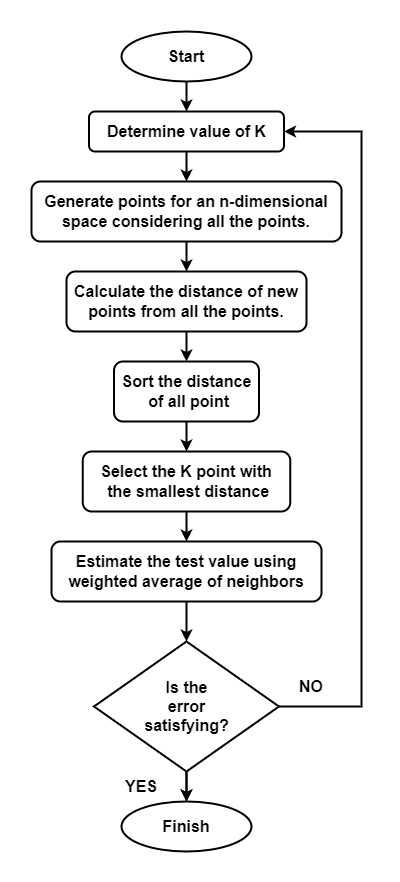
\includegraphics[width=\linewidth,height=200mm]{figures/KNN.png}
% \vspace{-25mm}
\caption{K-Nearest Neighbor (KNN)}
\label{fig:KNN}
\end{figure}

\textbf{1. Data representation:} The data must be represented in a multidimensional space, with each feature denoting a dimension, in order to use the KNN method. This is done in order to calculate the separation between two data points.

\textbf{2. Distance metric:} A distance metric, such as the Euclidean distance, Manhattan distance, or cosine similarity, is used to determine the separation between two data points. The type of data and the issue being solved determine which distance metric should be used.

\textbf{3. K value selection:} When making a forecast for a new data point, the K value denotes how many nearest neighbors will be considered. The K value you choose should strike a balance between underfitting and overfitting because it can have an impact on how well the KNN algorithm performs.

\textbf{4. Classification:} When classifying data, the KNN algorithm locates a new data point's K nearest neighbors and gives it the class label that is most prevalent among those neighbors. This strategy is referred to as a "majority vote."

\textbf{5. Regression:} The KNN algorithm employs this average to forecast a new data point in regression by averaging the values of the K nearest neighbors.

\textbf{6. Training and testing:} Since there is no need for a training step, the KNN method is regarded as a lazy learning algorithm. To create predictions for new data points, the system instead stores the complete training set. To assess the effectiveness of the algorithm, a different test set is employed.

\textbf{7. Pros and cons:} The KNN algorithm's key benefits are its simplicity and capacity for multi-class issues. Additionally, it is simple to understand and apply. On the other hand, the approach might not work well with high-dimensional data and may be slow for huge datasets. The algorithm's performance can also be significantly impacted by the K value and distance metric that are selected.
\\

\\



\section{Performance Analysis} 
Performance analysis of a machine learning model involves evaluating the model's effectiveness and efficiency in making predictions. The metrics that were used to analyze the performance of the aforementioned machine learning models are Accuracy, Precision, Recall, Sensitivity and F1 score. These metrics are used to analyze the model's overall performance and help to identify locations for improvement. Confusion matrix summarizes the model's performance by showing the number of true positive, false positive, true negative, and false negative predictions made by the model. These predictions from confusion matrix are used to calculate the required metrics. The performance metrics used are briefly discussed below.
\\
\textbf{Accuracy: } 
Accuracy is a commonly used metric to evaluate the performance of a machine learning model. It is defined as the ratio of the number of correct predictions made by the model to the total number of predictions made. It provides a good overall picture of the model's performance. Model accuracy is important to evaluate and monitor over time because it helps gauge the model's performance, including its ability to process, understand, and even forecast future events or outcomes [\cite{3_meth}]. The formula for accuracy is:

Accuracy = (Number of correct predictions) / (Total number of predictions)

where the number of correct predictions is the sum of True Positives (TP) and True Negatives (TN), and the total number of predictions is the sum of True Positives, False Positives (FP), False Negatives (FN), and True Negatives. While the accuracy of a model can range between 0\% and 100\%, there is no universal threshold that is used to determine if a model has “good” accuracy or not [\cite{4_meth}]. Instead, the accuracy of the model is typically compared to the accuracy of some baseline model. When the accuracy of the training dataset comes very high whereas the accuracy of the testing dataset becomes very low, it leads to the concept of overfitting. Overfitting implies that the created model is a great fit only for the trained dataset, but the worst fit for the test dataset.
\\
\textbf{Precision: } 
Precision measures the proportion of positive predictions made by the model that are actually correct. Precision can be calculated using the following formula:

Precision = (True Positives) / (True Positives + False Positives)

where True Positives (TP) are the number of correct positive predictions made by the model, and False Positives (FP) are the number of incorrect positive predictions made by the model. Precision is a good metric to use when the cost of false positive predictions is high, such as in medical diagnosis or fraud detection. A high precision score means that the model is good at avoiding false positive predictions, but it may miss some true positive cases. 
\\
\textbf{Recall: } %pinky
Recall, also referred to as the true positive rate or sensitivity, is a statistic used to assess how well a binary 
classification model is doing. It is determined as the ratio of the total number of true positive cases to the total 
number of true positive forecasts, i.e., the number of times the model correctly predicts positive (i.e., the number
of positive cases in the test set).
Mathematically, recall can be defined as:
\\
\centerline{Recall = True Positives / (True Positives + False Negatives)}


where False Negatives (FN) are cases where the model mistakenly predicts negative for an actual positive case and True 
Positives (TP) are cases where the model correctly predicts positive.When accurately recognizing positive cases is more important than accurately identifying negative ones (such as when detecting fraud, sickness, etc.), recall is a useful statistic to employ. As opposed to a low recall value, which suggests that the model is missing many positive cases, a high recall value shows that the model is effective at recognizing positive cases.
Recall is frequently used in conjunction with other measures, such as precision, to provide a more thorough understanding
 of how well a binary classification model is performing. The True Positive (TP) and False Negative (FN) values in a 
confusion matrix are used to determine recall.
\\
\textbf{Specificity } %pinky
A binary classification model's effectiveness is measured by a parameter called specificity, commonly referred to as the true negative rate. It is determined as the ratio of the total number of true negative cases to the total number of true negative forecasts, i.e., the number of times the model correctly predicts negative (i.e., the number of negative cases in the test set). Mathematically, specificity can be defined as:
\\
\centerline{Specificity = True Negatives / (True Negatives + False Positives)
}
When  more accurate recognition of negative situations is needed than positive cases (such as not labeling a healthy patient as having a sickness), specificity is an excellent statistic to employ. Low specificity values suggest that the model is making a lot of erroneous positive predictions, while high specificity values show that the model is effective at identifying negative cases. To acquire a fuller understanding of a binary classification model's performance, specificity is frequently used in conjunction with other measures like recall. The True Negative (TN) and False Positive (FP) values in a confusion matrix are used to calculate specificity.
\\
\textbf{F1 Score: } %pinky
The performance of a binary classification model is summarized by the F1 score, a statistic that combines precision and recall to produce a single result. It is described as the harmonic mean of accuracy and calibration.
\\
\centerline{Specificity = True Negatives / (True Negatives + False Positives)
}
True Positives (TP) are the instances in which the model correctly predicts a positive result, False Positives (FP) are the instances in which the model mistakenly predicts a positive result for a true negative result, and False Negatives (FN) are the instances in which the model mistakenly predicts a negative result for a true positive result.When both precision and recall are equally important, the F1 score is a useful metric to employ. It has a range of 0 to 1, with 0 denoting the lowest possible precision and recall and 1 denoting the best possible precision and memory. The True Positive (TP), False Positive (FP), and False Negative (FN) values in a confusion matrix can be used to calculate precision and recall. The performance of the model based on the precision and recall values can then be summarized by the F1 score, which can be calculated as a single value.
\\

\section{Visual Search}
Two approaches Deep learning and Ensemble learning are used to implement the visual search functionality of the proposed system. As two types of datasets are used therefore a total of 4 techniques are used. In the first two techniques, the selected models were trained separately through the transfer learning method. Different combinations of the selected models were trained through ensemble learning in the latter two techniques.
%pinky
\subsection{ Technique 1: Deep Learning-based Approach with Kaggle Dataset
}
Convolutional neural network (CNN) models VGG16, ResNet50, and MobileNet have all been pre-trained and have been trained on sizable picture datasets for tasks like image categorization. A pre-trained model is used as a starting point for a new assignment in the deep learning technique known as transfer learning. This strategy is well-liked in computer vision because it enables analysts and programmers to make use of the strength of previously trained models and modify them for new tasks.The pre-trained model is typically employed in transfer learning as a feature extractor, where the pre-trained model's layers are frozen and used to extract features from new data. The additional layers that are added to the model and trained to categorize the fresh data can then be fed with these features. While the pre-trained model already has important features that can be used for the new task, this procedure is quicker than training a new model from scratch.
\\
\\
For instance, in VGG16, the network's initial layers extract straightforward features like edges and lines, whereas its subsequent layers extract more intricate features like forms and textures. A new fully connected layer that is taught to classify the fresh data can take these attributes as inputs.The process of creating a VGG16 neural model, which consists of sequentially adding layers and connecting the output of one layer to the input of the next, begins with dataset partitioning and image preprocessing. The weights of the VGG16 layers and the custom dense layer are then optimized to reduce loss using iterations of the training data using the fit() function.
\\
\\
Similar to this, ResNet50 use residual blocks to solve the vanishing gradients issue that might arise during the training of very deep neural networks. A new fully connected layer for classification can be created using the pre-trained ResNet50 model as a feature extractor and the extracted features as inputs.Similar to before, dataset splitting and image processing are carried out here as well. While performing multiclass classification tasks, a fully connected classification layer with softmax activation is included. The modelres50 object is then passed the training and validation data along with the appropriate number of steps, and the fit() function is invoked. The verbose argument's value is set to 1 to show training progress. The History object that the fit() function provides includes details about the accuracy and loss throughout training and validation.
\\
\\
Google created MobileNet, a compact CNN architecture that is designed for mobile and embedded devices. The number of parameters in the network is greatly decreased while accuracy is maintained by using depthwise separable convolutions. MobileNet is a well-liked option for real-time image identification jobs on mobile devices and other embedded systems because of its speed and efficiency.As before, dataset partitioning and image processing were carried out. Following a Dropout layer, a BatchNormalization layer, a dense layer, and ReLU activation, the output of the base is sent to a GlobalAveragePooling2Dlayer. Lastly, a Dense layer and softmax activation are used to classify the output of the final BatchNormalization layer. The accuracy metric, categorical cross-entropy loss function, and Adam optimizer are all used in the model's construction. Calling the model's fit() method while specifying the training and validation data generators, the number of epochs, and a list of callbacks is how the training process is carried out. The input data is preprocessed and fed to the model in batches using the training and validation data generators.
\\
\subsection{Technique 2: Deep Learning-based Approach with Prepared Dataset}
The same image has been taken in several ways for the prepared dataset. The dataset is divided into three folders after creation: train, test, and validation. Validation and train folders are used for model training. The test accuracy is determined using the test folder. The same deep learning models used for the Kaggle dataset are used for training. Then, using input data, this dataset was trained and evaluated.
%amrin
\subsection{ Technique 3: Ensemble Learning-based Approach with Kaggle Dataset
} An ensemble-based machine learning classification approach has been used to give better search results. This is basically a technique where multiple models are combined to form a single predictive system. The main idea behind this technique is that several models working together can produce better results than a single model alone. This is because each individual model can capture different patterns in the data and combining their predictions can result in a more robust and accurate prediction. The individual models used in an ensemble should have diverse structures, be trained on different parts of the data, or use different algorithms. This diversity helps to reduce the overfitting and bias of a single model, leading to more accurate predictions. It can help to balance the bias-variance trade-off of individual models where bias refers to the tendency of a model to oversimplify the problem and miss important patterns in the data, while variance refers to the tendency of a model to fit to noise in the data. Ensemble learning can help to reduce variance by combining diverse models, while also reducing bias by aggregating their predictions. The predictions from the individual models are combined in some way, such as taking the average, voting, or weighting. The specific aggregation method depends on the type of ensemble learning used. Common ensemble methods include bagging, boosting, and stacking. In this technique, a bagging ensemble model was applied that trains multiple models independently on different subsets of the data, and then aggregate their predictions. There are several ways to aggregate the predictions, including taking the average of the predictions, taking a weighted average based on the performance of each model, taking the majority voting of all the models or using a meta-model to learn the relationship between the predictions and the target variable. The main idea behind bagging is to reduce the variance of a single model by combining predictions from multiple models that have been trained on different parts of the data. This reduces the chance that any single model will fit the data too closely and fail to generalize to new data. The final prediction is formed by aggregating the predictions from multiple models, which helps to further reduce overfitting and improve the stability and accuracy of the model.

\begin{figure} []
\centering
% \vspace{-30mm}
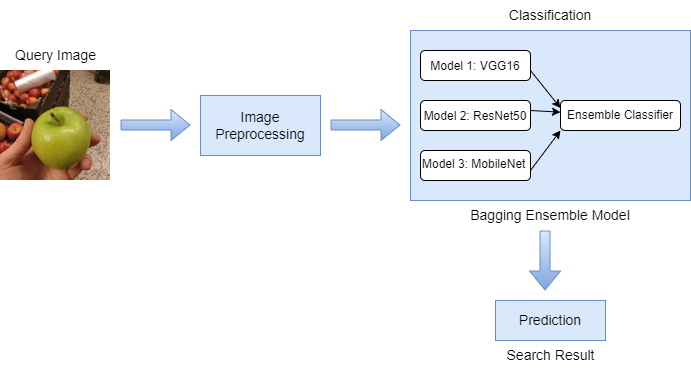
\includegraphics[width=150mm,height=120mm]{figures/ensemble1.png}
% \vspace{-25mm}
\caption{Ensemble Learning Model-1}
\label{fig:ensemble1}
\end{figure}
\begin{figure} [h]
\centering
% \vspace{-30mm}
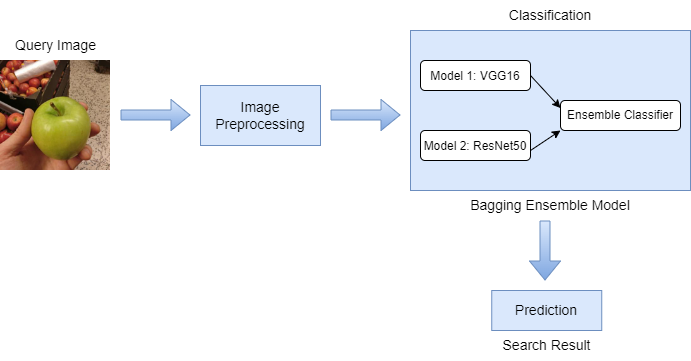
\includegraphics[width=150mm,height=120mm]{figures/ensemble2.png}
% \vspace{-25mm}
\caption{Ensemble Learning Model-2}
\label{fig:ensemble2}
\end{figure}

The individual classifiers taken in this approach are similar to the models used in the deep learning techniques above so that an accurate comparison could be made. Therefore VGG16, MobileNet, and ResNet50 this model are used. Four different ensemble learning models are built and used taking four different combinations of these three models. This is the technique using the Kaggle dataset. At first, splitting and preprocessing of the dataset is done. Then the selected models are trained on the training data. After that, each trained classifier is used to make predictions on new data which is the test data. The predictions from each classifier are combined taking the average of the predictions to make the final prediction. Averaging is a simple yet effective method of combining the predictions of multiple models in ensemble learning. In averaging, each individual model makes a prediction, and the final prediction is the average or mean of all the predictions. The main advantage of averaging is its simplicity. Averaging requires no additional training or optimization, and it can be used with any type of model. Additionally, averaging can reduce the variance of the predictions, resulting in a more stable and robust final prediction. It may not work well if the individual models have very different levels of accuracy but here the selected models have shown somewhat the same level of accuracy. 

\begin{figure} []
\centering
% \vspace{-30mm}
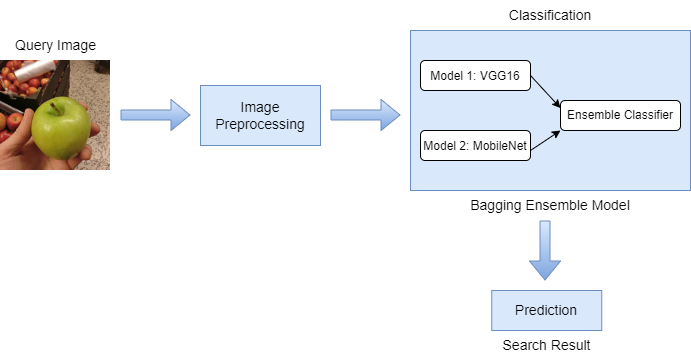
\includegraphics[width=150mm,height=120mm]{figures/ensemble3.png}
% \vspace{-25mm}
\caption{Ensemble Learning Model-3}
\label{fig:ensemble3}
\end{figure}
\begin{figure} []
\centering
% \vspace{-30mm}
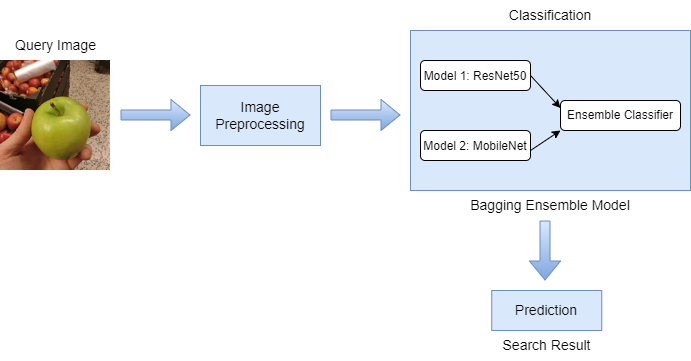
\includegraphics[width=150mm,height=120mm]{figures/ensemble4.png}
% \vspace{-25mm}
\caption{Ensemble Learning Model-4}
\label{fig:ensemble4}
\end{figure}

Therefore the input to this bagging ensemble model is the set of training data with input features and a target variable. The output of each individual model in the bagging ensemble is a predicted class label. The final prediction is the majority vote or average of all the class labels predicted by the individual models. VGG16, MobileNet, and ResNet50 all three models are combined in the first ensemble learning model as seen in Fig.\ref{fig:ensemble1}. VGG16 and ResNet50 in the second model [Fig.\ref{fig:ensemble2}], VGG16 and MobileNet in third model [Fig.\ref{fig:ensemble3}] and MobileNet and ResNet50 in fourth model [Fig.\ref{fig:ensemble4}] are used. So this system works by taking a query or search image followed by its preprocessing and classification where the ensemble classifier combines the predictions of the individual trained classifiers and the final prediction is shown as the visual search result.





\subsection{ Technique 4: Ensemble Learning-based Approach with Prepared Dataset}
With this technique, the entire process of technique 3 is repeated. However, in this case, the prepared dataset has been used instead of the Kaggle dataset. In the first ensemble learning model, VGG16, MobileNet, and ResNet50 are all merged as seen in Fig.\ref{fig:ensemble1}. VGG16 and ResNet50 in the second model  [Fig.\ref{fig:ensemble2}], VGG16 and MobileNet in the third model [Fig.\ref{fig:ensemble3}], and MobileNet and ResNet50 in the fourth model [Fig.\ref{fig:ensemble4}] have been used.

%naw
\section{Product Recommendation}
After reviewing many of the algorithms that are popular for image recommendation, two seemed to be the perfect fit for implementing the product recommendation part: K means clustering and K-Nearest Neighbor (KNN). Here K means clustering is used as the pre-processing step and after that KNN is applied to get product recommendations. Along with these two models, the models that were used in product recognition were used as well.



 These models have been used separately and combined through ensemble learning to find out the combination with the best results. An elaborate description of these models is given below.



\section{Technique 1: Machine learning Approach with Kaggle Dataset}

For this technique, there are three combinations available. The combinations are as follows -\\
i. VGG-16 and KNN Approach\\
ii. ResNet50 and KNN Approach\\
iii. MobileNet and KNN Approach\\

\begin{figure} [H]
\centering
% \vspace{-30mm}
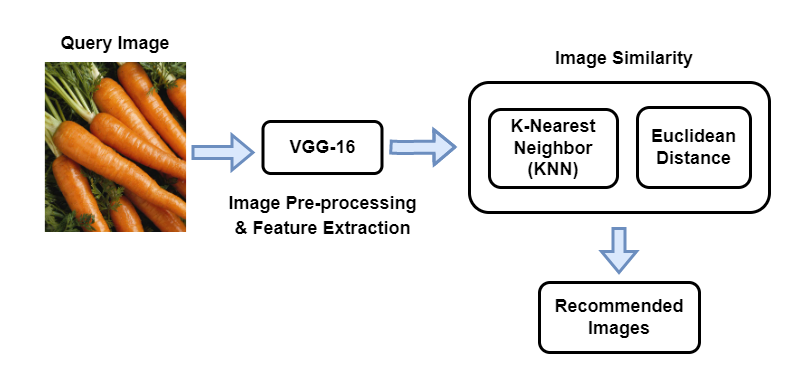
\includegraphics[width=\linewidth,height=80mm]{figures/VggKNN.png}
% \vspace{-25mm}
\caption{VGG-16 and KNN Approach}
\label{fig:VggKNN}
\end{figure}

\begin{figure} [H]
\centering
% \vspace{-30mm}
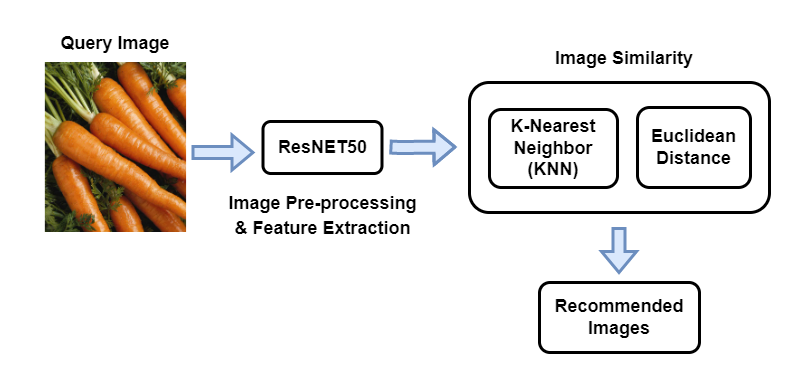
\includegraphics[width=\linewidth,height=80mm]{figures/Res50KNN.png}
% \vspace{-25mm}
\caption{ResNet50 and KNN Approach}
\label{fig:ResKNN}
\end{figure}

\begin{figure} [H]
\centering
% \vspace{-30mm}
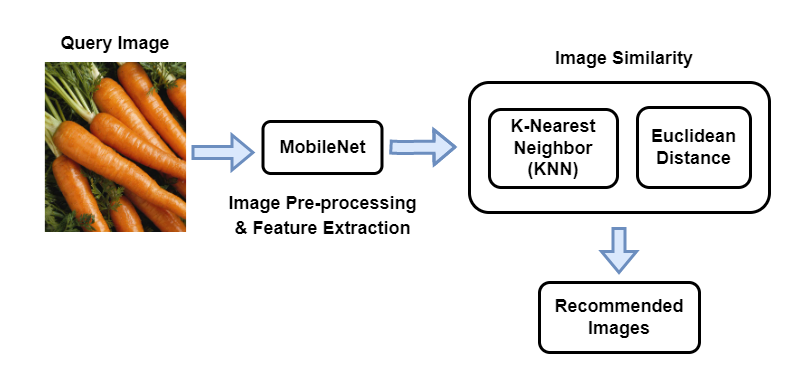
\includegraphics[width=\linewidth,height=80mm]{figures/MobileKNN.png}
% \vspace{-25mm}
\caption{MobileNet and KNN Approach}
\label{fig:MobKNN}
\end{figure}

Going through these three combinations, the first combination consists of VGG-16 and KNN. Here VGG-16 is used as the preprocessing and feature extraction step. After the preprocessing and feature extraction, KNN was applied to determine image similarity and give recommended images as output [Fig.\ref{fig:VggKNN}]. Similarly, the second and third combinations are built using ResNet50 [Fig.\ref{fig:ResKNN}] and Mobilenet [Fig.\ref{fig:MobKNN}]  respectively as the image preprocessing and feature extraction step in the place of VGG-16. After the individual application of pre-processing and feature extraction steps, KNN has been applied to all of the combinations. This will lead to an output of ten images which are the recommended images.

Here KNN compares each image's attributes, such as color, texture, shape, and other visual qualities. Then, based on the similarity between the attributes in each image, it determines the k-nearest neighbors. Then, recommendations are made using these k-nearest neighbors [Fig.\ref{fig:KNN}].



\section{Technique 2: Machine learning Approach with Prepared Dataset}

With this technique, the entire process of technique 1 is repeated. However, here the technique will be applied to the prepared dataset instead of the Kaggle dataset. All three combinations mentioned earlier will be used here as well. The three mentioned algorithms such as VGG-16, RedNet50, and MobileNet will be used as the preprocessing and feature extraction respectively for the three combinations. After the completion of preprocessing and feature extraction on the prepared dataset, KNN will be applied. An output of ten images will be generated.  [Fig.\ref{fig:VggKNN}], [Fig.\ref{fig:ResKNN}], [Fig.\ref{fig:MobKNN}]

\section{Technique 3: Ensemble learning Approach with Kaggle Dataset}


With this technique, there exists four combinations and they are as follows -\\
i. Ensemble Model 1 (VGG-16, ResNet50, MobileNet) and KNN Approach\\
ii. Ensemble Model 2 (VGG-16, ResNet50) and KNN Approach\\
iii. Ensemble Model 3 (VGG-16, MobileNet) and KNN Approach\\
iv. Ensemble Model 4 (ResNet, MobileNet) and KNN Approach\\

\begin{figure} [H]
\centering
% \vspace{-30mm}
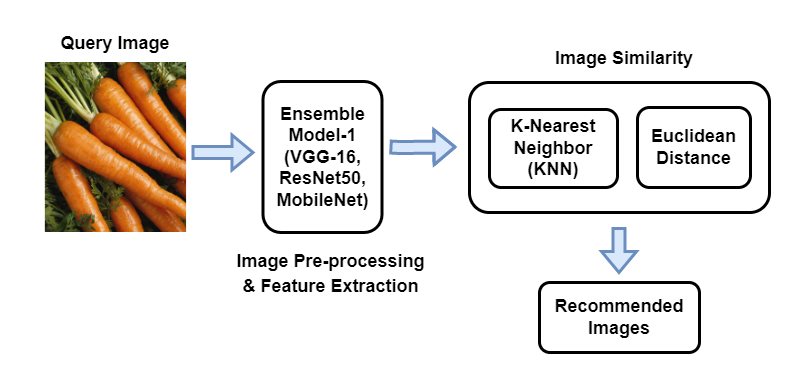
\includegraphics[width=\linewidth,height=80mm]{figures/E1_KNN.png}
% \vspace{-25mm}
\caption{ Ensemble Model 1 (VGG-16, ResNet50, MobileNet) and KNN Approach}
\label{fig:E1KNN}
\end{figure}

\begin{figure} [H]
\centering
% \vspace{-30mm}
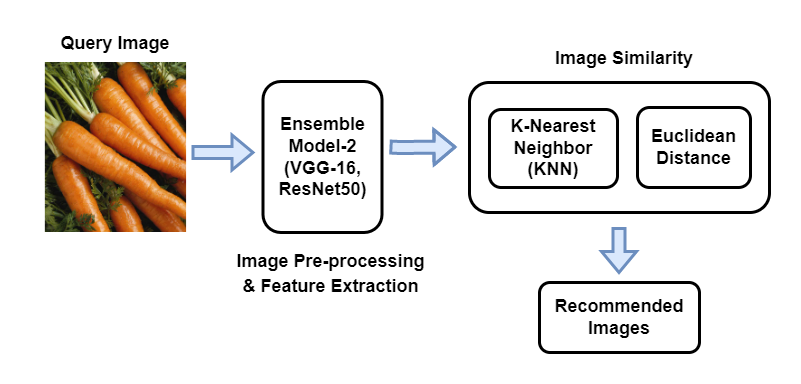
\includegraphics[width=\linewidth,height=80mm]{figures/E2_KNN.png}
% \vspace{-25mm}
\caption{ Ensemble Model 2 (VGG-16, ResNet50) and KNN Approach}
\label{fig:E2KNN}
\end{figure}


\begin{figure} [H]
\centering
% \vspace{-30mm}
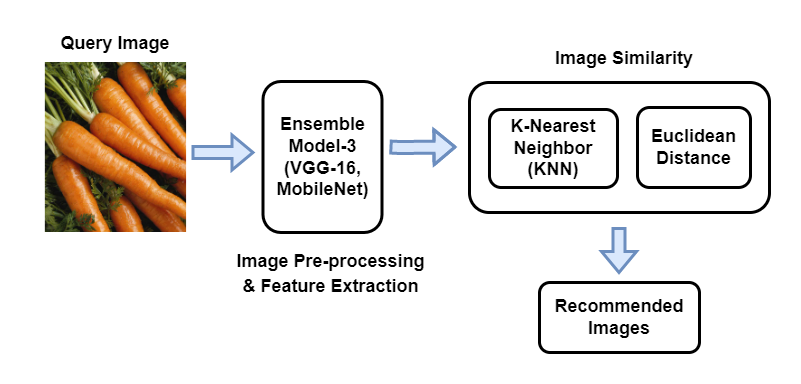
\includegraphics[width=\linewidth,height=80mm]{figures/E3_KNN.png}
% \vspace{-25mm}
\caption{ Ensemble Model 3 (VGG-16, MobileNet) and KNN Approach}
\label{fig:E3KNN}
\end{figure}

\begin{figure} [H]
\centering
% \vspace{-30mm}
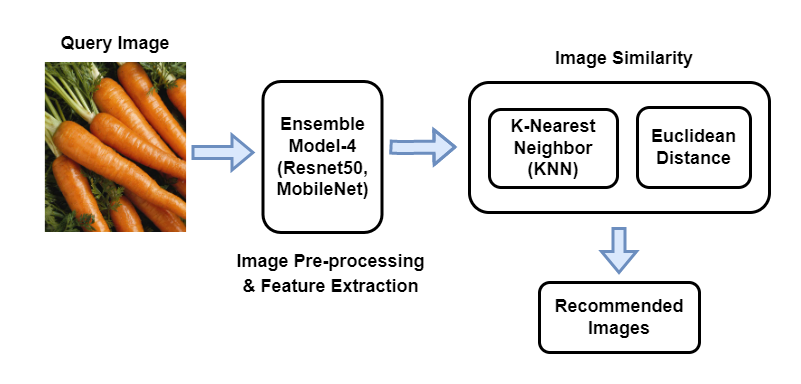
\includegraphics[width=\linewidth,height=80mm]{figures/E4_KNN.png}
% \vspace{-25mm}
\caption{ Ensemble Model 4 (ResNet, MobileNet) and KNN Approach}
\label{fig:E4KNN}
\end{figure}

Considering the first combination out of the four chosen combinations. It consists of ensemble model-1 and KNN. Here, ensemble model-1 is used for preprocessing and feature extracting from Kaggle dataset. Ensemble model-1 consists of VGG-16 [Fig.\ref{fig:vgg16}], ResNet50 [Fig.\ref{fig:resnet}], and MobileNet[Fig.\ref{fig:mobilenet}]. After the completion of this step, KNN is applied to the processed dataset which gives ten images as recommended images.\\

Similarly, the second combination consists of ensemble model-2 and KNN. Here ensemble model-2 is used for preprocessing and feature extracting from the Kaggle dataset. Ensemble model-2 consists of VGG-16 [Fig.\ref{fig:vgg16}] and ResNet50 [Fig.\ref{fig:resnet}]. After the completion of this site, KNN is applied to the processed dataset which again gives ten images as recommended images.\\

Familiar steps are followed for both the third and fourth combinations. Ensemble model-3 and ensemble model-4 are applied respectively for combination 3 and combination 4 for preprocessing and feature extraction. After this, KNN is applied to both of the combinations to generate recommended images individually for the two combinations.

\section{Technique 4: Ensemble Learning Approach with Prepared Dataset}

With this technique, the process of technique 3 is repeated all over again. The four combinations mentioned before are used here to achieve the desired recommended images. The four combinations are ensemble model-1,2,3 and 4 for preprocessing and feature extraction respectively. After the preprocessing and feature extraction step, KNN is applied to each of the combinations. However, the dataset used here is the prepared dataset.

%naw
\end{comment}  
\endinput

